\documentclass[11pt,a4paper]{article}
\usepackage[margin=2.2cm]{geometry}
\usepackage{lmodern}
\usepackage{graphicx}
\usepackage{booktabs}
\usepackage{amsmath}
\usepackage{siunitx}
\usepackage{microtype}
\usepackage[hidelinks]{hyperref}
\usepackage[numbers,sort&compress]{natbib}
\usepackage{caption}
\usepackage{enumitem}
\usepackage{placeins}
\renewcommand{\topfraction}{0.9}\renewcommand{\bottomfraction}{0.7}\renewcommand{\textfraction}{0.08}\renewcommand{\floatpagefraction}{0.75}
\setcounter{topnumber}{3}\setcounter{totalnumber}{5}
\usepackage{tabularx}
\usepackage{wasysym}
\captionsetup{font=small,labelfont=bf}
\sisetup{per-mode=symbol,range-phrase=--,range-units=single}
\DeclareSIUnit\rev{rev}
\graphicspath{{./figures/}}

\title{\textbf{FlexTome: a 3D-printed, flexure-pivot rocking microtome with a differential-screw feed for \SI{5}{\micro\metre} paraffin histology at a \$60 bill of materials}}
\author{Design report: Engineering Mechanics / Biomedical Engineering}
\date{}

\begin{document}
\maketitle

\begin{abstract}
Histopathology is the reference standard for cancer diagnosis, but much of sub-Saharan Africa has roughly one pathologist per million people and district hospitals lack the US\$150\,000--200\,000 of equipment an essential pathology laboratory requires. The microtome that cuts 3--\SI{5}{\micro\metre} paraffin sections is one of the few items in that chain with no low-cost substitute: new manual rotary microtomes list at US\$9\,000--22\,700, and the thinnest published open-source sectioning device cuts at $\geq$\SI{50}{\micro\metre}, an order of magnitude too thick for diagnostic H\&E. We present FlexTome, a rocking-arm microtome designed to be printed on a \SI{235}{\milli\metre} desktop FDM printer and completed with hardware-store fasteners. Three design decisions make \SI{5}{\micro\metre} sectioning plausible from printed plastic: (i)~the arm pivot is a cross-strip flexure built from three \SI{0.20}{\milli\metre} spring-steel feeler-gauge strips, so the metrology loop contains no sliding or rolling joint and therefore no backlash; (ii)~the \SI{5}{\micro\metre} feed is generated by a differential screw (M8$\times$1.25 against M8$\times$1.0, \SI{0.25}{\milli\metre} per revolution) indexed by a 50-tooth printed ratchet that the arm itself advances at the top of each stroke, so the micrometre-scale motion is carried entirely by steel threads while the printed parts need only millimetre tolerances; and (iii)~the disposable blade rides on a monolithic printed parallelogram flexure stage preloaded against the screw. A crank-rocker drive gives a \SI{54}{\milli\metre} arc stroke at $\pm$\ang{12.5}. An analytic structural-loop model, calibrated by plane-stress finite-element models of the flexure stage and of the frame, predicts a feed-axis loop stiffness of \SI{1.0}{\newton\per\micro\metre}; the frame model caught a \SI{0.83}{\micro\metre\per\newton} tower compliance that the beam model had missed and drove a gusset revision that cut it to \SI{0.21}{\micro\metre\per\newton}. A Monte-Carlo budget combining thread-pitch error, printed-ratchet error, cutting-force variation, pawl seating and thermal drift predicts a section thickness of $5.0\pm0.6$\,\si{\micro\metre} (1~s.d.; 90\,\% interval 4.1--\SI{5.9}{\micro\metre}) at the \SI{5}{\micro\metre} setting, comparable to the $>\pm10\,\%$ deviation measured on commercial rotary microtomes in a 154-site survey. All structural resonances ($\geq$\SI{357}{\hertz}) lie far above the $<$\SI{10}{\hertz} cutting excitation, so chatter is not predicted. The bill of materials is US\$60.39, a $>99\,\%$ reduction relative to new list price. The design, analysis code and a validation protocol are released so that the predictions can be tested on a physical build.
\end{abstract}

\section{Introduction}
\subsection{The problem}
The cancer-diagnosis chain in low- and middle-income countries (LMICs) fails at the laboratory before it fails at the clinic. A 2016 survey of African pathology resources found population-per-pathologist ratios from 84\,000 (Mauritius) to 9.3~million (Niger), against 15\,000--20\,000 in the UK and US~\citep{Nelson2016}; the Lancet Commission on diagnostics estimates that 47\,\% of the world's population has little or no access to diagnostics~\citep{Fleming2021}; and an essential district-hospital pathology package costs US\$150\,000--200\,000 in equipment~\citep{Fleming2016}. Within that package, the microtome is the only instrument that converts a fixed, paraffin-embedded biopsy into the 3--\SI{5}{\micro\metre} section a pathologist can read. New manual rotary microtomes list at US\$22\,690 (Leica RM2125 RTS), US\$21\,548 (Sakura Accu-Cut SRM~200) and US\$8\,995 (Thermo HM~325); used units sell for US\$2\,100--7\,950 (vendor prices, October 2026).

\subsection{Why no low-cost microtome exists}
Open-source hardware has reached the microscope: the OpenFlexure microscope is printed for US\$20--200 and has been manufactured locally in Tanzania and Kenya~\citep{Collins2020}. It has not reached the microtome. The published low-cost sectioning devices cut at $\geq$\SI{50}{\micro\metre} (a hair-clipper vibrating razor~\citep{Bazer1980}), $<$\SI{100}{\micro\metre} for hand-fed plant tissue (Rapid-Tome~\citep{Thomas2023}) and \SI{250}{\micro\metre}--\SI{1}{\milli\metre} for live organoids (a US\$853 HardwareX slicer~\citep{MartinezMartin2024}). None embeds in paraffin, none uses a standard disposable microtome blade, and none has a micrometre-resolution feed. The barrier is mechanical: a \SI{5}{\micro\metre} section demands that the knife-to-specimen distance repeat to better than $\sim$\SI{1}{\micro\metre} stroke after stroke, while printed plastic parts have $\pm$0.1--\SI{0.2}{\milli\metre} dimensional scatter~\citep{Melenka2015}, creep under sustained load~\citep{Waseem2020}, a Young's modulus 60 times lower than steel~\citep{Tymrak2014}, and sliding joints printed in plastic have backlash of tens of micrometres.

\subsection{The design thesis}
Our thesis is that these limitations can be designed around rather than overcome, using three principles from precision-instrument design:
\begin{enumerate}[nosep]
\item \textbf{No sliding joints in the metrology loop.} Every joint between the blade edge and the specimen face that must repeat to $<$\SI{1}{\micro\metre} is a flexure: the arm pivot is a cross-strip flexure, the blade stage is a parallelogram flexure, and the screw-to-stage interface is a preloaded nut. Flexures have zero backlash and no stick-slip~\citep{Smith2000,Wittrick1948}.
\item \textbf{Keep the micrometre chain in steel.} The feed increment (\SI{5}{\micro\metre}) is set by the pitch difference of two standard steel threads and the tooth count of a ratchet; the printed parts only hold those steel parts in roughly the right place. The differential screw turns a \SI{0.25}{\milli\metre} pitch difference into fine motion without a precision thread~\citep{SmithChetwynd2017}.
\item \textbf{Make the structural loop short and deep.} Section-to-section thickness variation equals loop compliance $\times$ cutting-force variation; chatter is a stiffness phenomenon~\citep{Bayley1955,Warshawsky1983}. The loop is a one-piece ribbed base and a gusseted tower whose root depth (\SI{60}{\milli\metre}) was set by finite-element analysis.
\end{enumerate}
The rocking-arm kinematics themselves are not new: Horace Darwin's 1885 Cambridge rocker used a pivoted arm, screw feed and ratchet, and a modified rocker later cut sections for electron microscopy~\citep{Eaves1954}. What is new is the realisation of that kinematic in printed plastic and commodity steel at a \$60 bill of materials, with an explicit, FE-checked stiffness and error budget.

\FloatBarrier
\section{Design}
\subsection{Architecture}
Figure~\ref{fig:concept} shows the assembly. The coordinate frame has $x$ along the feed (specimen~$\rightarrow$~blade), $y$ along the blade edge and $z$ vertical. Table~\ref{tab:subsystems} summarises the subsystems.

\begin{figure}[!htbp]\centering
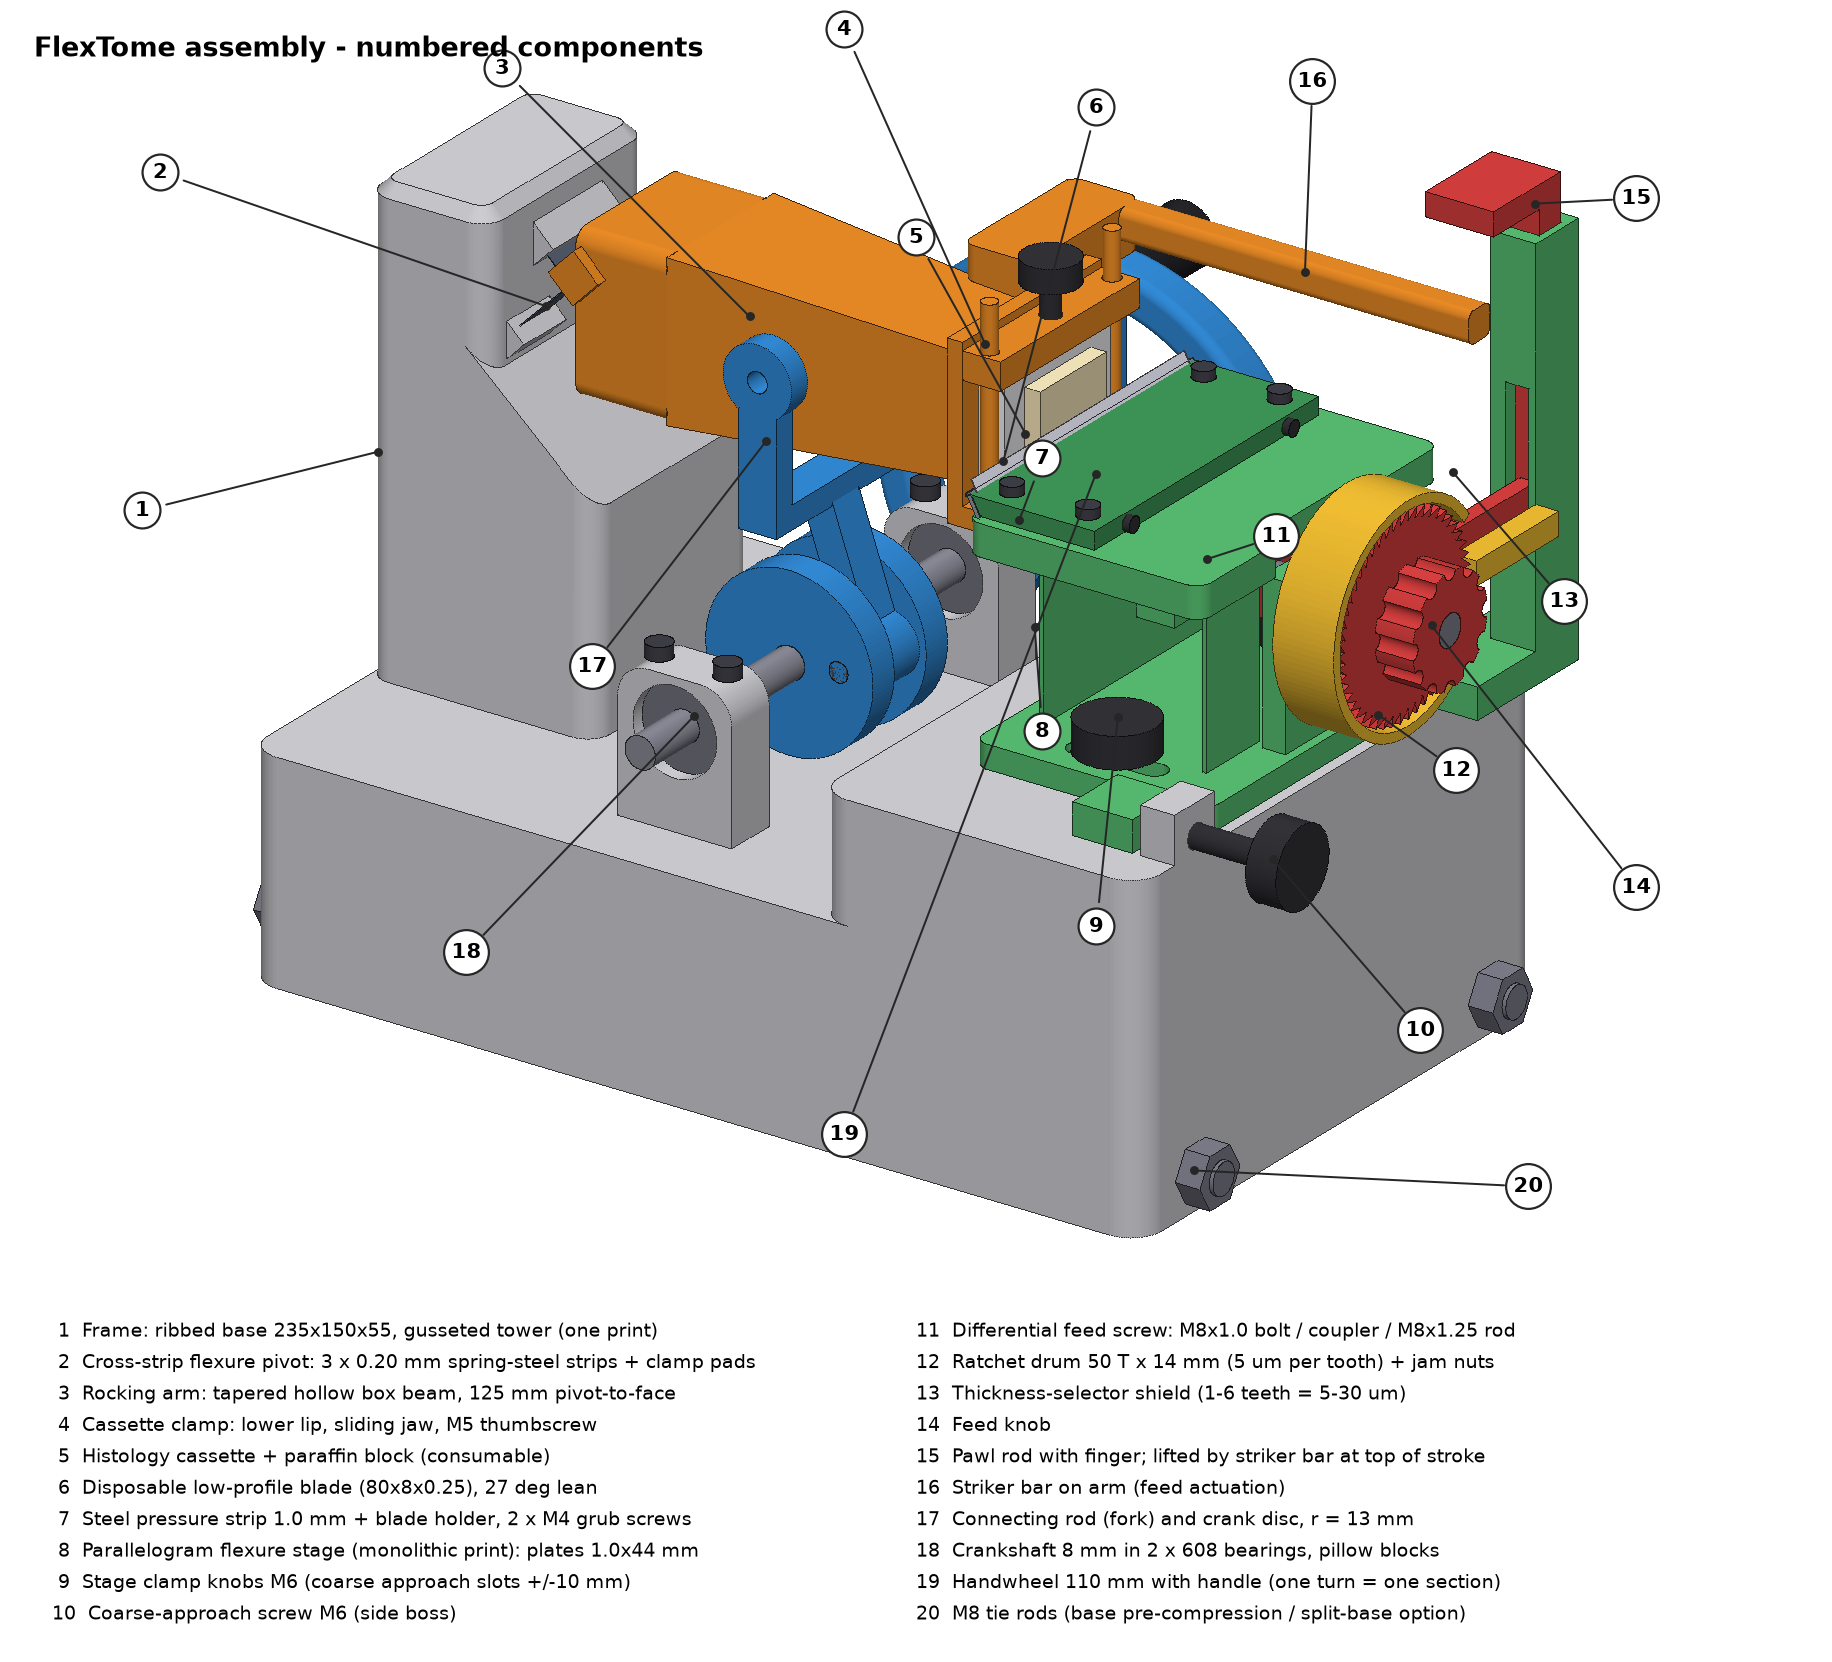
\includegraphics[width=\linewidth]{fig1_assembly_callouts.png}
\caption{FlexTome assembly with numbered components (frame footprint $235\times150$\,mm; overall envelope $272\times210\times202$\,mm including handwheel, feed knob and pawl rod). The specimen in a standard histology cassette (5) is carried on a \SI{125}{\milli\metre} printed arm (3) that rocks $\pm$\ang{12.5} on a cross-strip steel flexure pivot (2). The blade (6) sits on a parallelogram flexure stage (8) driven along $x$ by a differential screw (11); a striker bar on the arm (16) lifts a pawl rod (15) at the top of each stroke, advancing the 50-tooth ratchet drum (12) by 1--6 teeth (5--\SI{30}{\micro\metre}) as set by the selector shield (13). A crank-rocker (17, 18) with 608 bearings and a \SI{110}{\milli\metre} handwheel (19) drives the arm. Rendered from the parametric CAD model; Sec.~\ref{sec:mech} walks through each subsystem.}
\label{fig:concept}
\end{figure}

\begin{table}[!htbp]\small\centering
\caption{Subsystems and their role in the error budget.}
\label{tab:subsystems}
\begin{tabularx}{\linewidth}{@{}p{2.0cm}XX@{}}
\toprule
Subsystem & Implementation & Role in the error budget \\
\midrule
Frame & One printed part: $235\times150\times55$\,mm ribbed base, \SI{118}{\milli\metre} tower with a forward gusset (\SI{60}{\milli\metre} root depth tapering to \SI{32}{\milli\metre} at the pivot head), raised front deck; two M8 steel tie rods through the base & Closes the structural loop (\SI{0.21}{\micro\metre\per\newton} pivot-to-deck by FE); tie rods pre-compress the print against creep/warp and allow a split base for small printers \\
Arm pivot & Cross-strip flexure: three strips (10/20/10\,mm wide) of \SI{0.20}{\milli\metre} feeler-gauge steel, \SI{20}{\milli\metre} free length, crossing at mid-length, clamped in printed pads with M3 screws & Zero backlash; axially stiff (\SI{40}{\newton\per\micro\metre}); rotational stiffness \SI{0.27}{\newton\metre\per\radian} \\
Arm & Tapered hollow box beam $40\rightarrow30$\,mm, \SI{125}{\milli\metre} pivot-to-face; integral cassette clamp (fixed lower lip, sliding jaw, M5 thumbscrew) & Loaded axially during the cut; \SI{0.08}{\micro\metre\per\newton} \\
Drive & Crank radius \SI{13}{\milli\metre} at \SI{60}{\milli\metre} from pivot, crank centre \SI{71.2}{\milli\metre} below the arm joint; \SI{71.2}{\milli\metre} fork connecting rod running between two printed crank webs; built-up crankshaft of two \SI{8}{\milli\metre} stubs in two 608 bearings; \SI{110}{\milli\metre} spoked handwheel & Kinematics only; not in the metrology loop \\
Blade stage & Monolithic printed parallelogram: two $1.0\times44$\,mm plates (60\,mm and $2\times20$\,mm wide), platform, hanging nut tab; bolted to deck through slots ($\pm$\SI{10}{\milli\metre} coarse approach) & Guides the blade along $x$ with no sliding; pitch stiffness carries the cutting moment \\
Blade holder & Disposable low-profile blade ($80\times8\times0.25$\,mm) leaning back \ang{27} from vertical; \SI{1.0}{\milli\metre} steel pressure strip in front, two M4 grub screws from behind; \SI{2.5}{\milli\metre} edge overhang & Clearance angle \ang{9.5} nominal; overhang compliance \SI{0.25}{\micro\metre\per\newton} \\
Fine feed & Differential screw: M8$\times$1.0 bolt in the stage-tab nut, joined by a printed coupler to an M8$\times$1.25 rod in the frame nut $\rightarrow$ \SI{0.25}{\milli\metre\per\rev} stage motion while the screw itself translates \SI{1.25}{\milli\metre\per\rev}; \SI{14}{\milli\metre} long 50-tooth ratchet drum keeps the pawl engaged over the $\pm$\SI{5}{\milli\metre} screw travel; sector shield on the column selects 1--6 teeth; stage travel $\pm$\SI{1}{\milli\metre} (400 sections at \SI{5}{\micro\metre}) per reset & Sets the increment; thread-pitch scatter \SI{0.37}{\micro\metre} (1~s.d.) \\
Feed actuation & Vertical pawl rod in a printed guide, lifted $\leq$\SI{22}{\milli\metre} by a striker bar fixed to the arm during the last $\sim$\ang{6} of the upstroke; gravity/spring return & Feed occurs at top dead centre, after the return stroke \\
\bottomrule
\end{tabularx}
\end{table}

\subsection{Kinematics}
The crank-rocker (Fig.~\ref{fig:kin}a,b; Sec.~\ref{sec:mech}) gives $\theta=\pm$\ang{12.5}, a block-face stroke of \SI{54}{\milli\metre} and a peak cutting speed of \SI{174}{\milli\metre\per\second} at 60~rpm, one section per handwheel turn. Because the specimen travels on an arc, the face retracts \SI{3.0}{\milli\metre} from the blade at the stroke ends and the cut face is a cylinder of radius \SI{125}{\milli\metre} (sagitta \SI{0.40}{\milli\metre} over a \SI{20}{\milli\metre} block). The latter is the rocker's classical ``curved section'' property; because every stroke follows the identical arc, the curvature is cut into the block face once and the next section (the difference between two successive arcs) has uniform thickness. The effective clearance angle varies by $\pm$\ang{4.6} across a \SI{20}{\milli\metre} face; a \ang{27} blade lean (clearance \ang{9.5} at mid-face, rake \ang{45.5} with a \ang{35} blade facet) keeps it within 4.9--\ang{14.1}, inside the 3--\ang{15} range practitioners recommend (Fig.~\ref{fig:kin}c).

\begin{figure}[!htbp]\centering
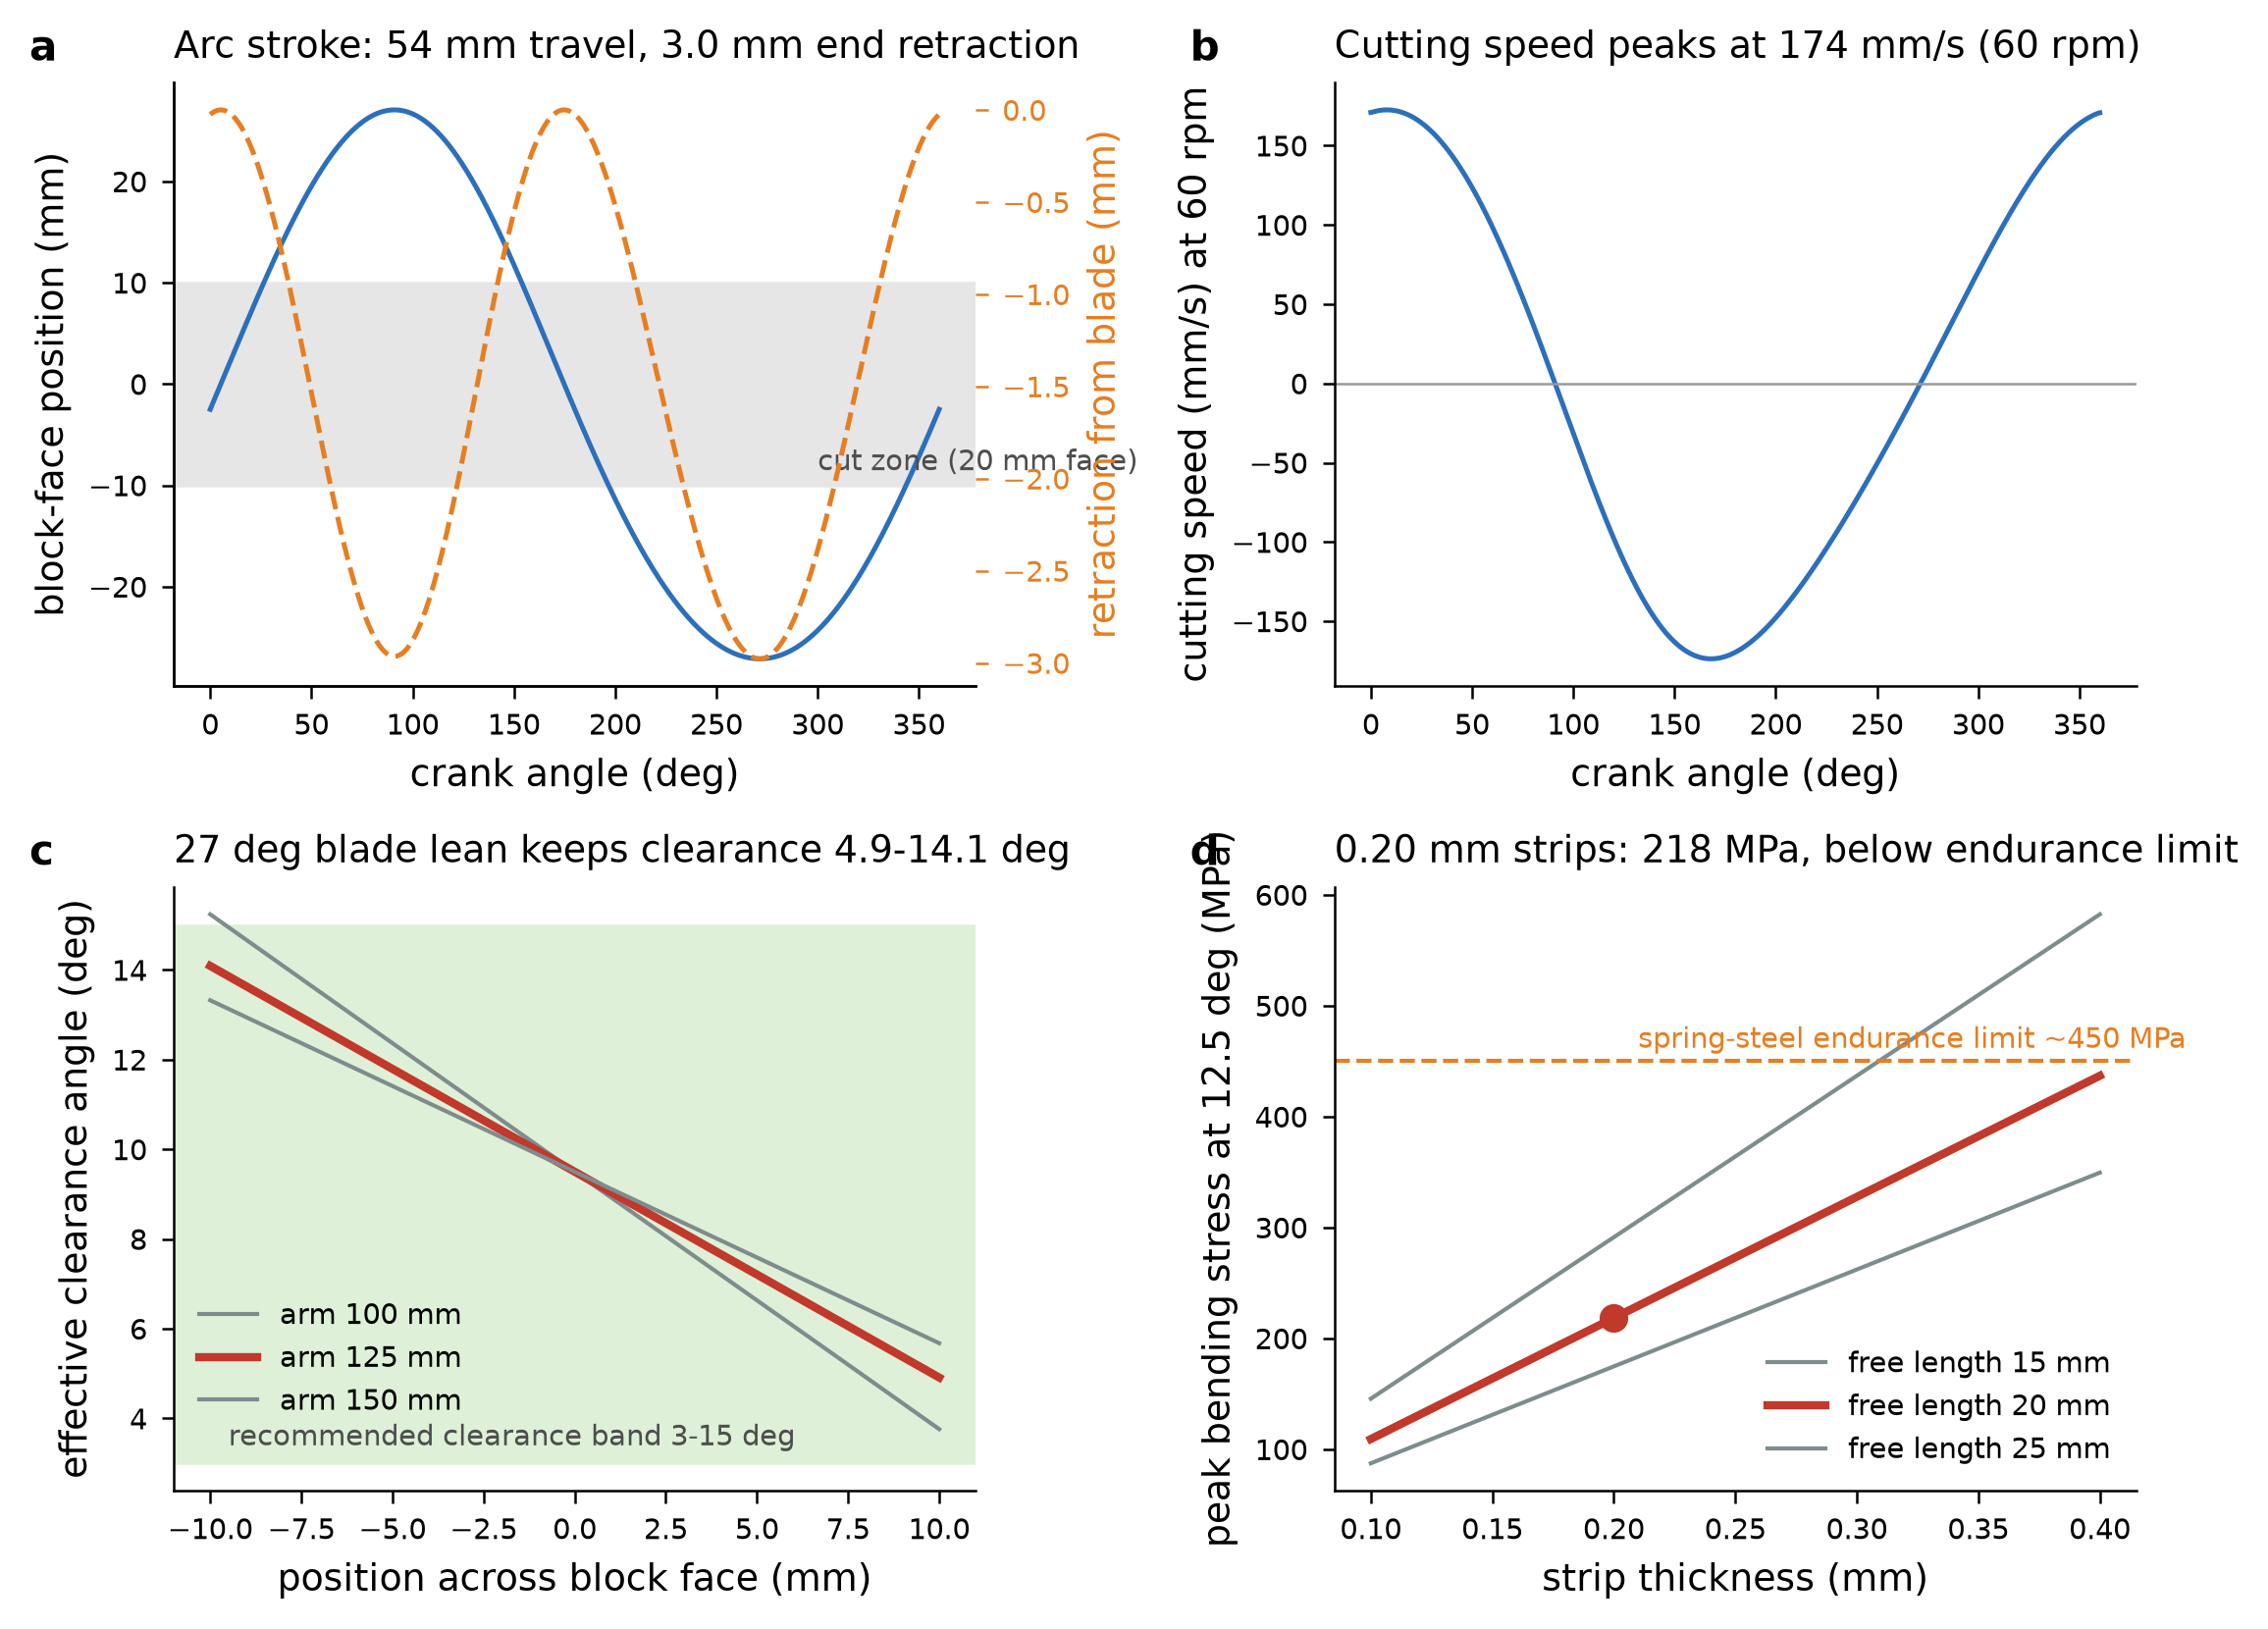
\includegraphics[width=\linewidth]{fig2_kinematics_pivot.png}
\caption{Kinematics and pivot. (a)~Face position and retraction vs crank angle. (b)~Cutting speed. (c)~Effective clearance angle across the face for three arm lengths. (d)~Peak pivot-strip bending stress vs strip thickness; the chosen $0.20\times20$\,mm strips reach \SI{218}{\mega\pascal} at full swing, below the $\sim$\SI{450}{\mega\pascal} endurance limit of hardened spring steel (feeler-gauge stock; the exact limit must be taken from the stock datasheet). Rotational stiffness is \SI{0.267}{\newton\metre\per\radian} (torque \SI{0.058}{\newton\metre} at full swing); the second-order centre shift is $\approx0.1\,L\theta^2\approx$\SI{95}{\micro\metre} at $\pm$\ang{12.5}, which is repeatable and therefore shapes the arc rather than the thickness~\citep{Wittrick1948,Haringx1949}.}
\label{fig:kin}
\end{figure}

\subsection{Feed resolution}
With pitches $p_1=\SI{1.25}{\milli\metre}$ and $p_2=\SI{1.00}{\milli\metre}$, one revolution advances the stage by $p_1-p_2=\SI{0.25}{\milli\metre}$ toward the specimen; one tooth of the 50-tooth ratchet is \SI{5.0}{\micro\metre}. The selector shield exposes $k=1\ldots6$ teeth to the pawl, giving 5, 10, 15, 20, 25 or \SI{30}{\micro\metre} settings (trimming at 20--\SI{30}{\micro\metre}, sectioning at \SI{5}{\micro\metre}). Only the \emph{difference} of the two threads matters, so ordinary rolled-thread hardware is sufficient: the budget assumes 1\,\% independent local pitch error on each thread and \SI{3}{\micro\metre} peak-to-peak periodic error per revolution.

\subsection{Blade stage design}
Figure~\ref{fig:stage}a maps plate thickness and height against bending stress at the $\pm$\SI{1}{\milli\metre} feed travel and against the $x$-stiffness that sets the preload. The chosen $1.0\times44$\,mm plates give $k_x=\SI{4.9}{\newton\per\milli\metre}$ (analytic) / \SI{4.0}{\newton\per\milli\metre} (FE), $\leq$\SI{5}{\newton} preload on the screw, \SI{5.4}{\mega\pascal} peak plate stress and a creep safety factor of 2.8 against a \SI{15}{\mega\pascal} sustained-stress limit for PLA~\citep{Waseem2020}; PETG or ASA are drop-in alternatives. In the screw-held condition the stage is a short cantilever about the nut; the FE model (Fig.~\ref{fig:feastage}) gives \SI{0.109}{\micro\metre\per\newton} at the blade edge, half the analytic estimate, and this value is used in the budget.

A consequence of the differential principle that is easy to overlook: the screw body advances through the frame nut by the full \SI{1.25}{\milli\metre} per revolution while the stage moves \SI{0.25}{\milli\metre}, so over the $\pm$\SI{1}{\milli\metre} stage range the screw, coupler, ratchet and knob translate $\pm$\SI{5}{\milli\metre}. The ratchet is therefore a \SI{14}{\milli\metre} drum rather than a wheel, the coupler sits in a \SI{26}{\milli\metre} gap between the stage tab and the frame nut, and the thickness-selector shield is mounted on the stage body, not on the screw. A boolean interference audit of the assembly (Sec.~\ref{sec:audit}) confirmed that no unintended contacts remain over the full stroke and screw travel.

\begin{figure}[!htbp]\centering
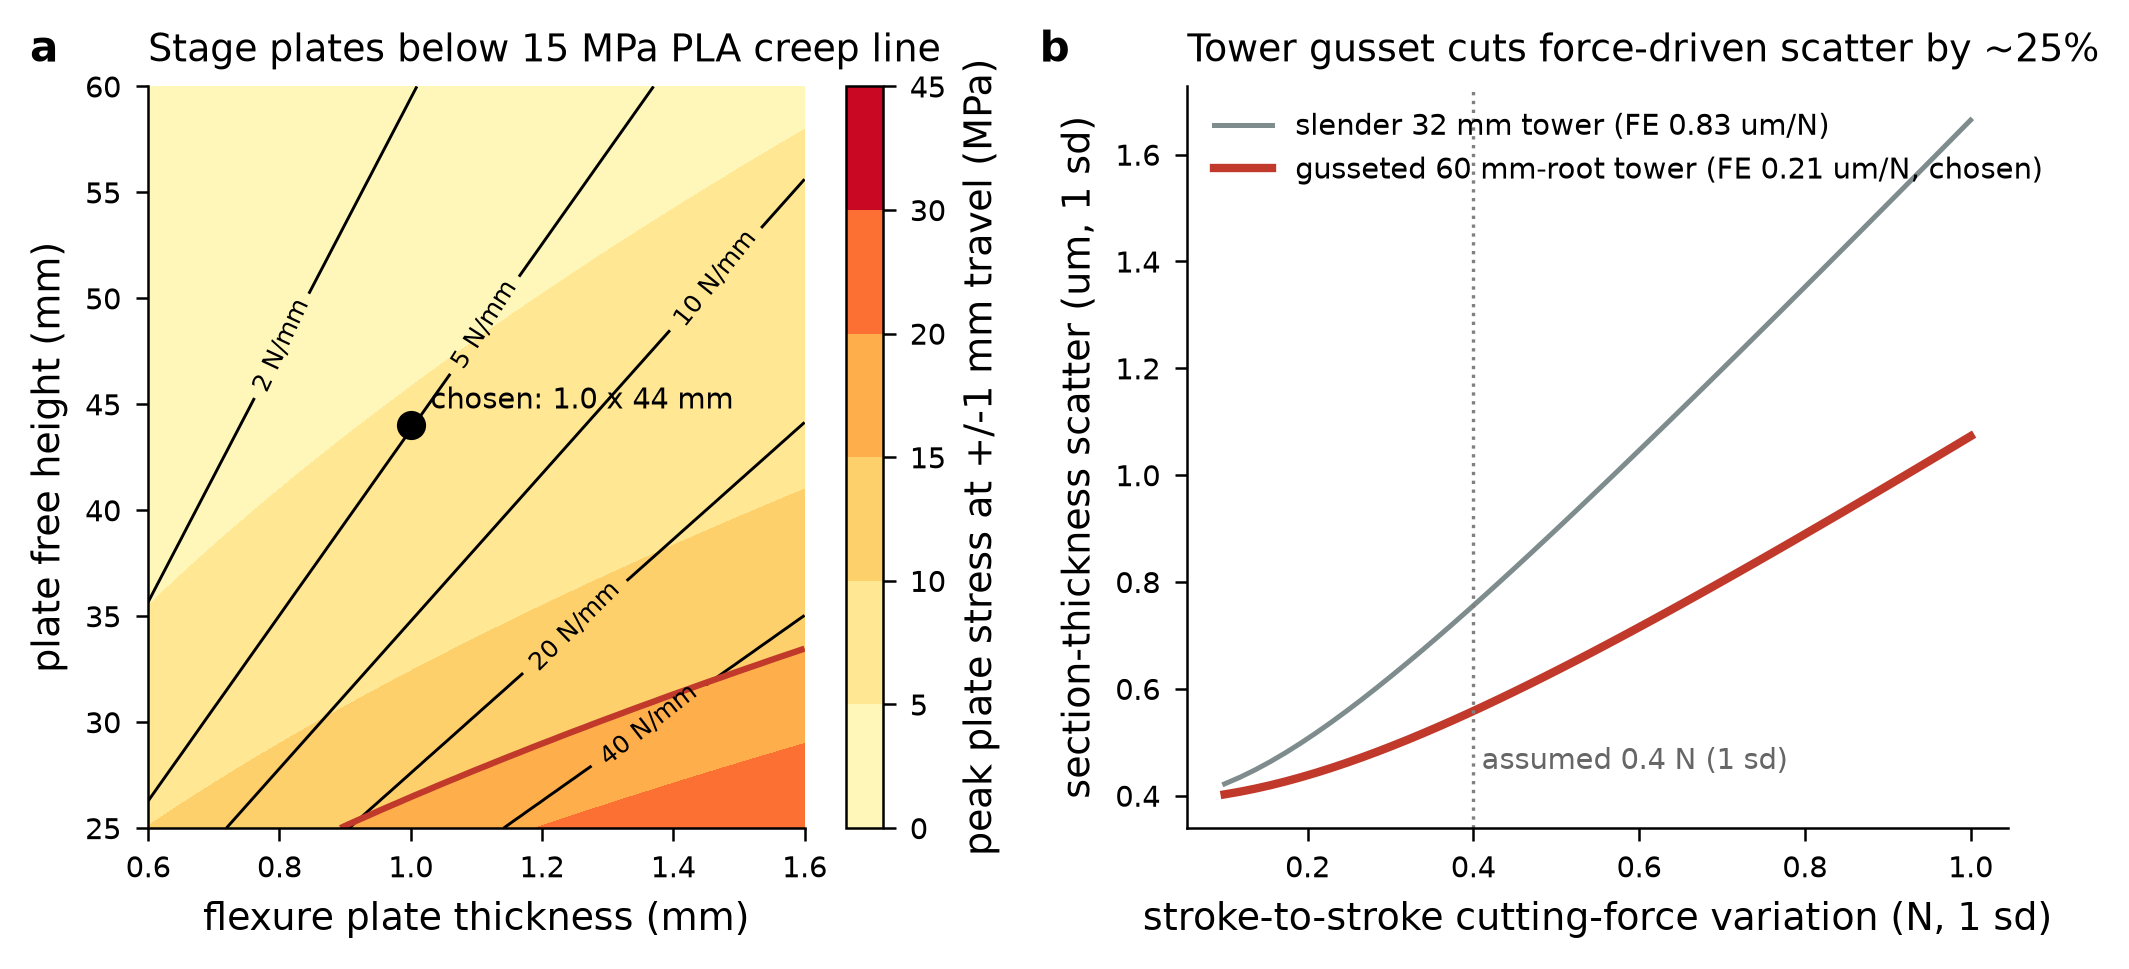
\includegraphics[width=\linewidth]{fig4_stage_design_map.png}
\caption{(a)~Design map of the flexure stage; the red contour is the \SI{15}{\mega\pascal} PLA creep line. (b)~Predicted thickness scatter vs cutting-force variation for the original slender tower and the gusseted tower; the gusset reduces scatter by $\sim$25\,\% at the assumed \SI{0.4}{\newton} force variation.}
\label{fig:stage}
\end{figure}

\begin{figure}[!htbp]\centering
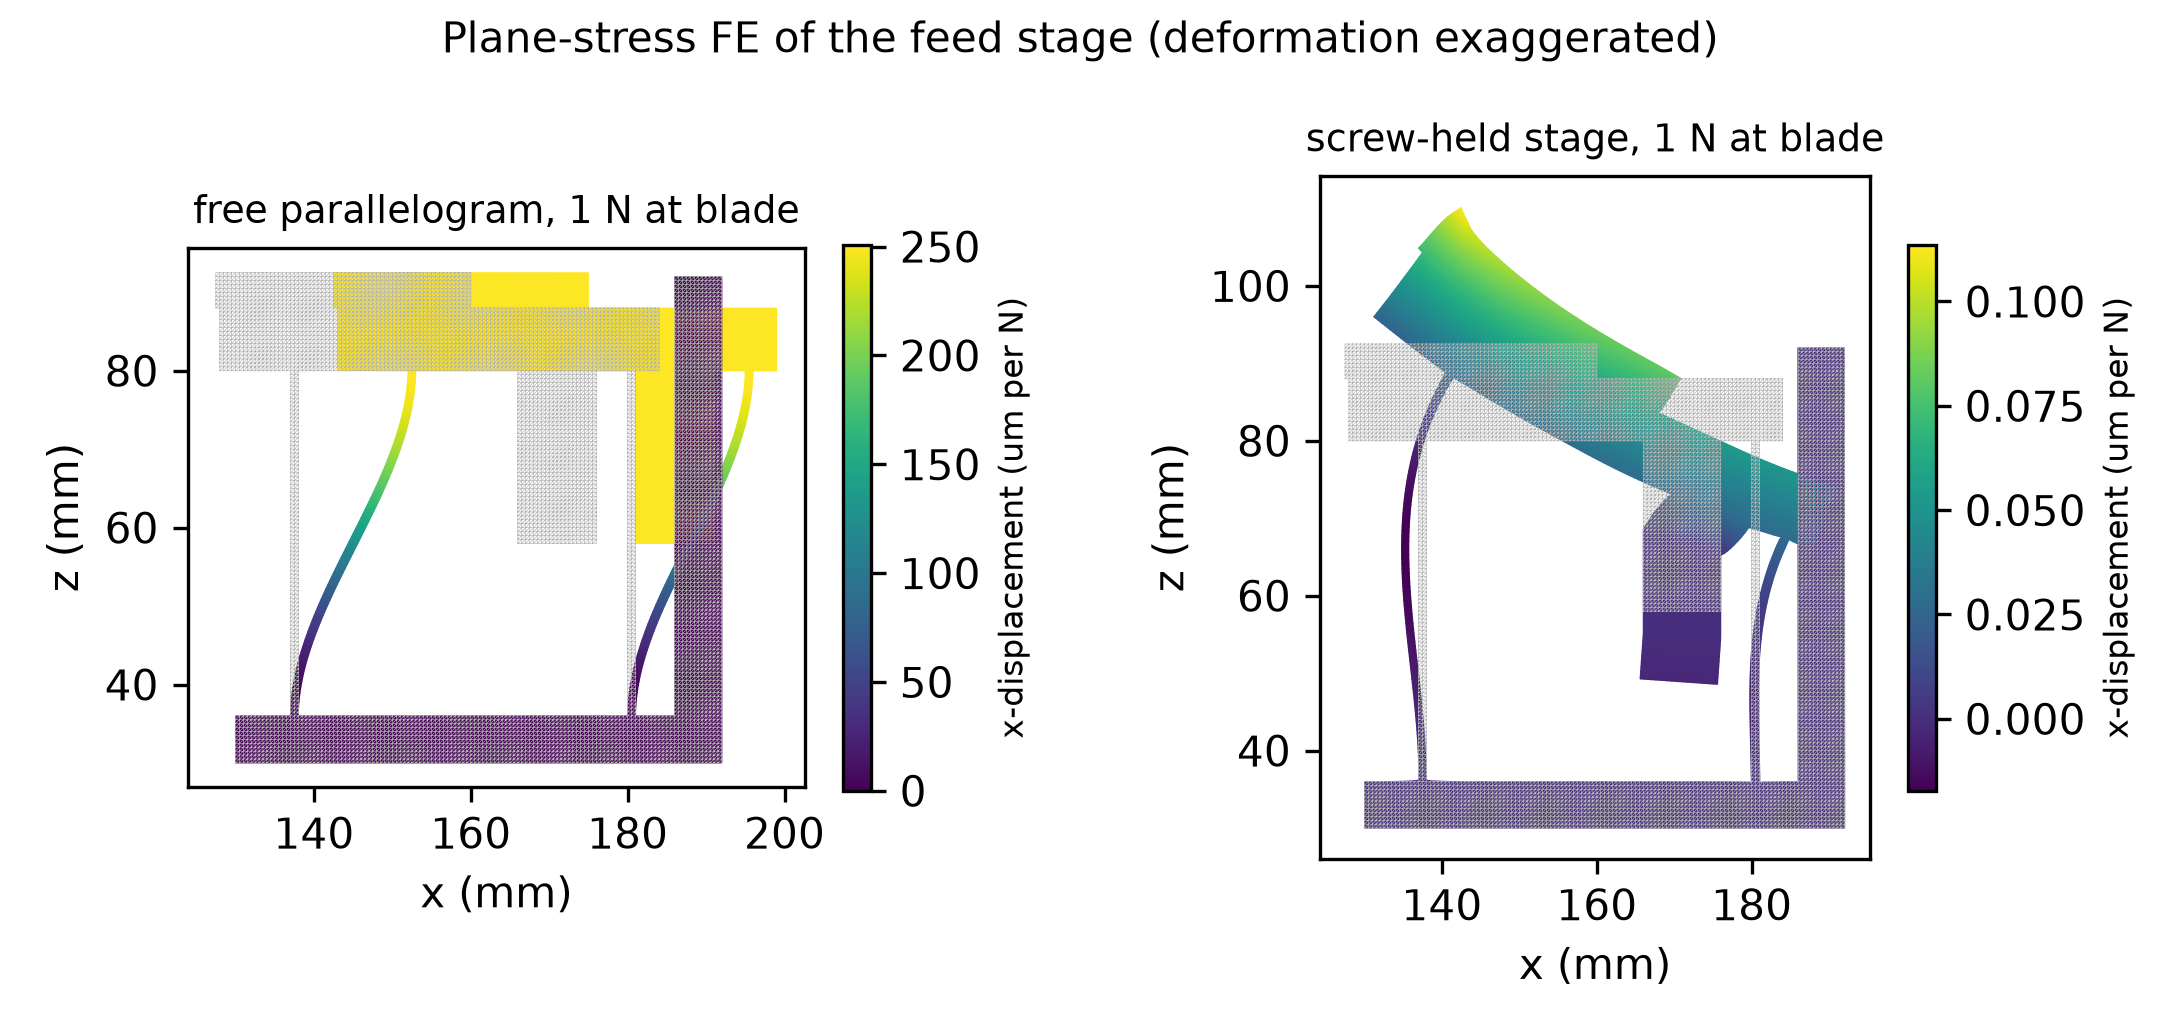
\includegraphics[width=\linewidth]{fig5_fea_stage.png}
\caption{Plane-stress finite-element model (scikit-fem, quadratic triangles, 12\,882 elements; out-of-plane widths represented by scaling $E$ per region). Left: free stage under \SI{1}{\newton} at the blade, $k_x=\SI{3.99}{\newton\per\milli\metre}$. Right: stage held at the nut, compliance \SI{0.109}{\micro\metre\per\newton} at the blade.}
\label{fig:feastage}
\end{figure}

\subsection{Frame design: an FE-driven revision}
The beam model treated the tower as a $70\times70$\,mm box and the base as a plate rotating under the tower-root moment, and predicted that two M8 tie rods would triple base rigidity. A plane-stress FE model of the frame side-section (Fig.~\ref{fig:feaframe}) showed otherwise: with the tower as actually drawn (\SI{32}{\milli\metre} deep), pivot-to-deck compliance was \SI{0.83}{\micro\metre\per\newton}, essentially all tower bending, and the tie rods changed it by only 2\,\% because the ribbed base was already stiff. Adding a forward gusset (the tower root widened to \SI{60}{\milli\metre} over the first \SI{55}{\milli\metre} of height, tapering to the \SI{32}{\milli\metre} head, within the existing footprint and clear of the arm's swing) reduced the frame compliance to \SI{0.21}{\micro\metre\per\newton}. The tie rods were retained for a different reason: they pre-compress the printed base against creep and warp and allow the base to be printed in two halves on small printers.

\begin{figure}[!htbp]\centering
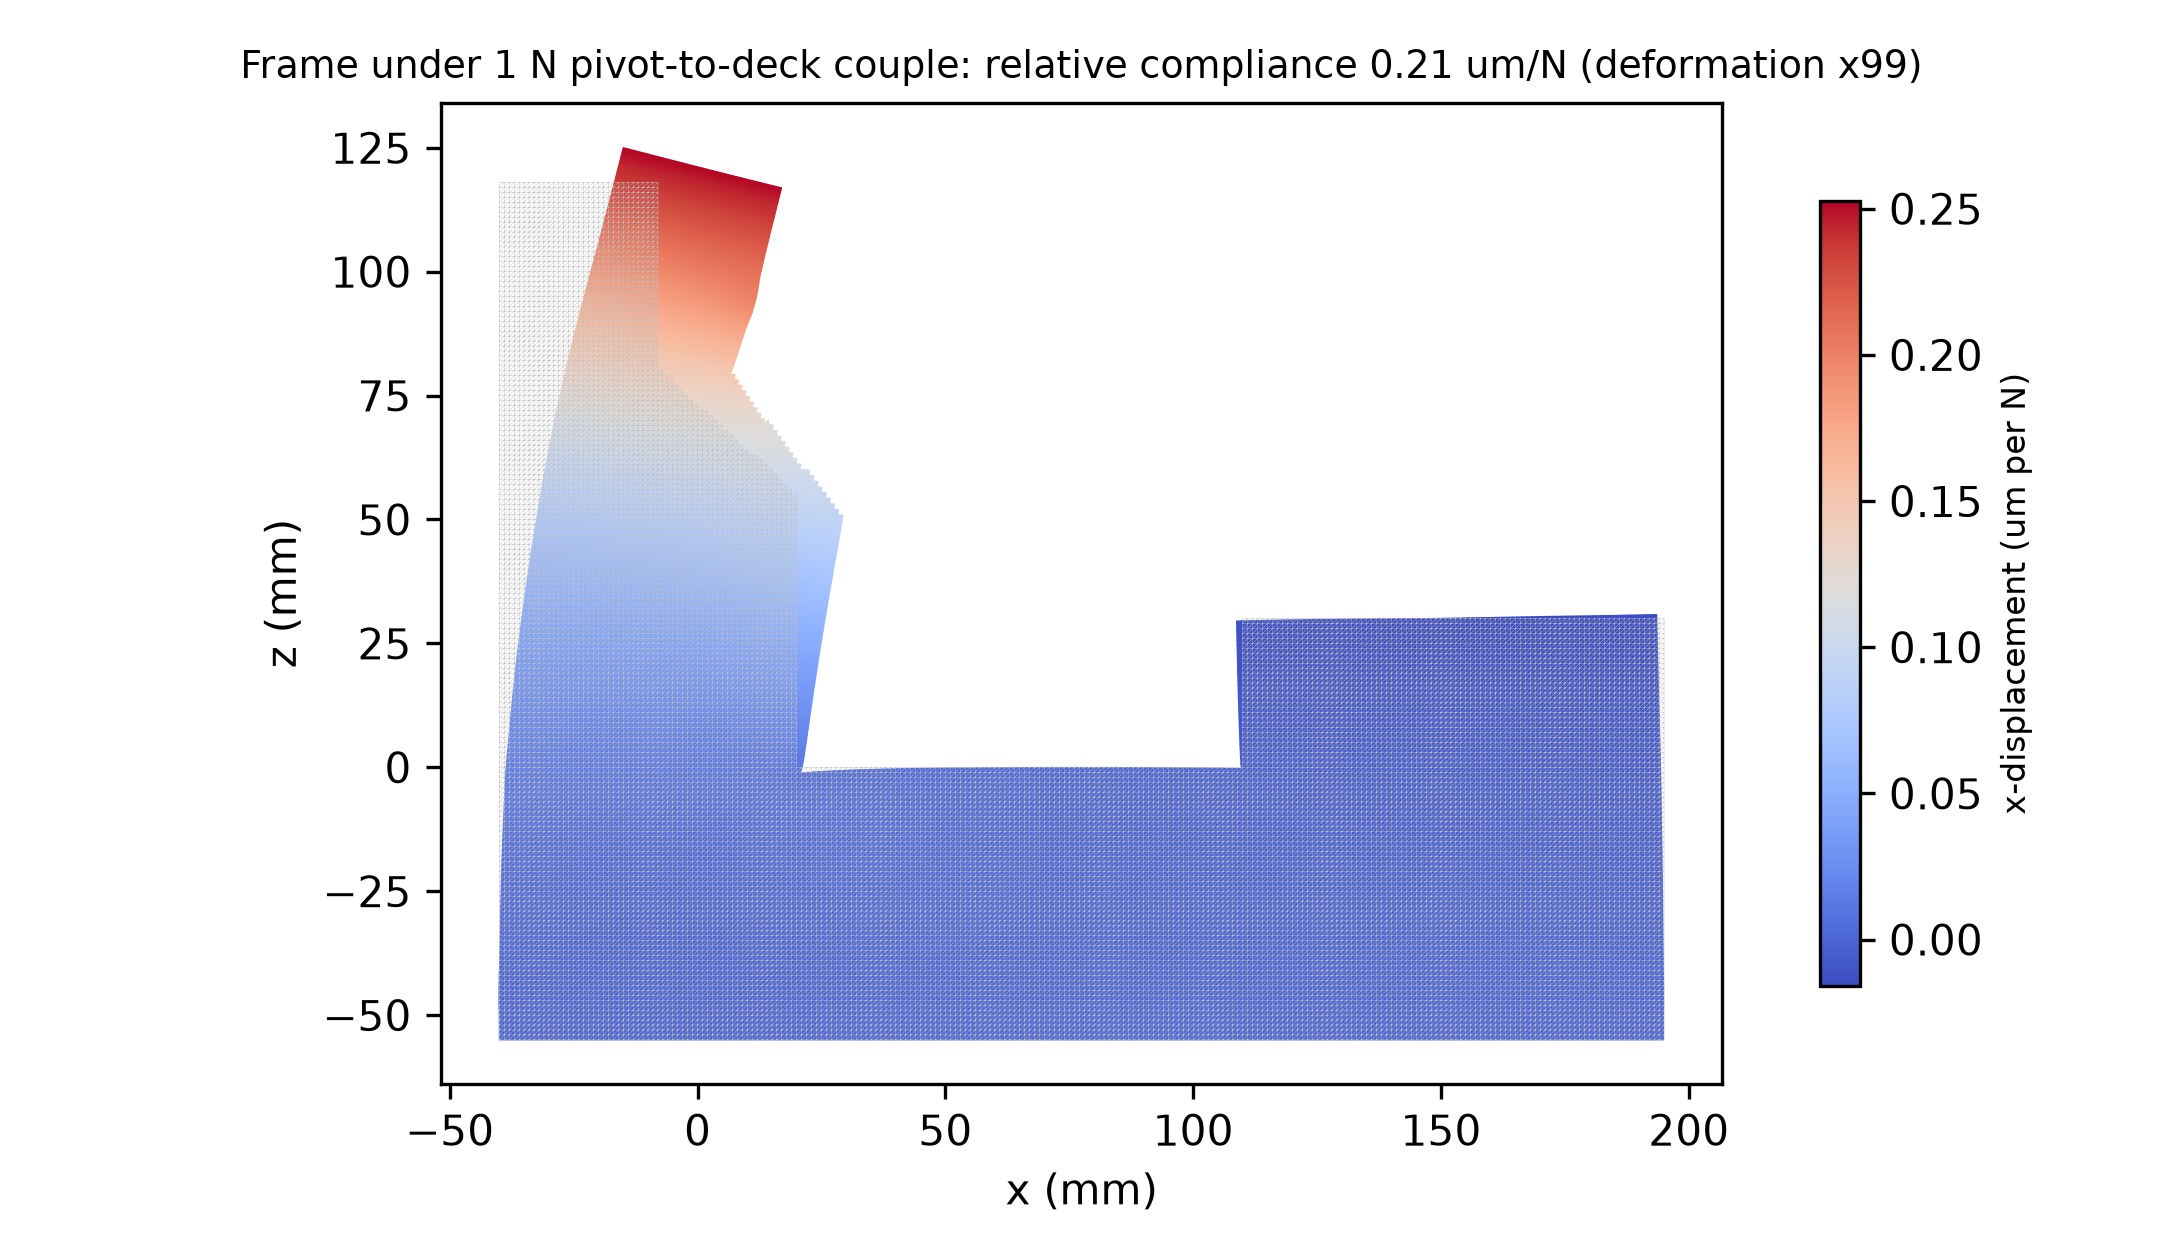
\includegraphics[width=0.9\linewidth]{fig6_fea_frame.png}
\caption{Plane-stress FE of the gusseted frame under a self-equilibrated \SI{1}{\newton} couple between the pivot and the stage-foot clamp zone (quadratic triangles, 42\,281 elements; ribbed base represented by a 40\,\% web fraction with solid \SI{6}{\milli\metre} skins). Relative pivot-to-deck compliance \SI{0.21}{\micro\metre\per\newton}, versus \SI{0.83}{\micro\metre\per\newton} for the original slender tower.}
\label{fig:feaframe}
\end{figure}

\section{Mechanism walkthrough}
\label{sec:mech}
This section follows the machine from the handwheel to the section ribbon, naming every part (Fig.~\ref{fig:concept}, numbered 1--20; Fig.~\ref{fig:section}, cut at $y=0$) and giving the governing relation for each stage with the numbers used in the design. Throughout, $x$ is the feed axis (specimen~$\rightarrow$~blade), $y$ runs along the blade edge, $z$ is up, and the pivot axis is the $y$-parallel line through $P=(0,0,95)$\,mm.

\begin{figure}[!htbp]\centering
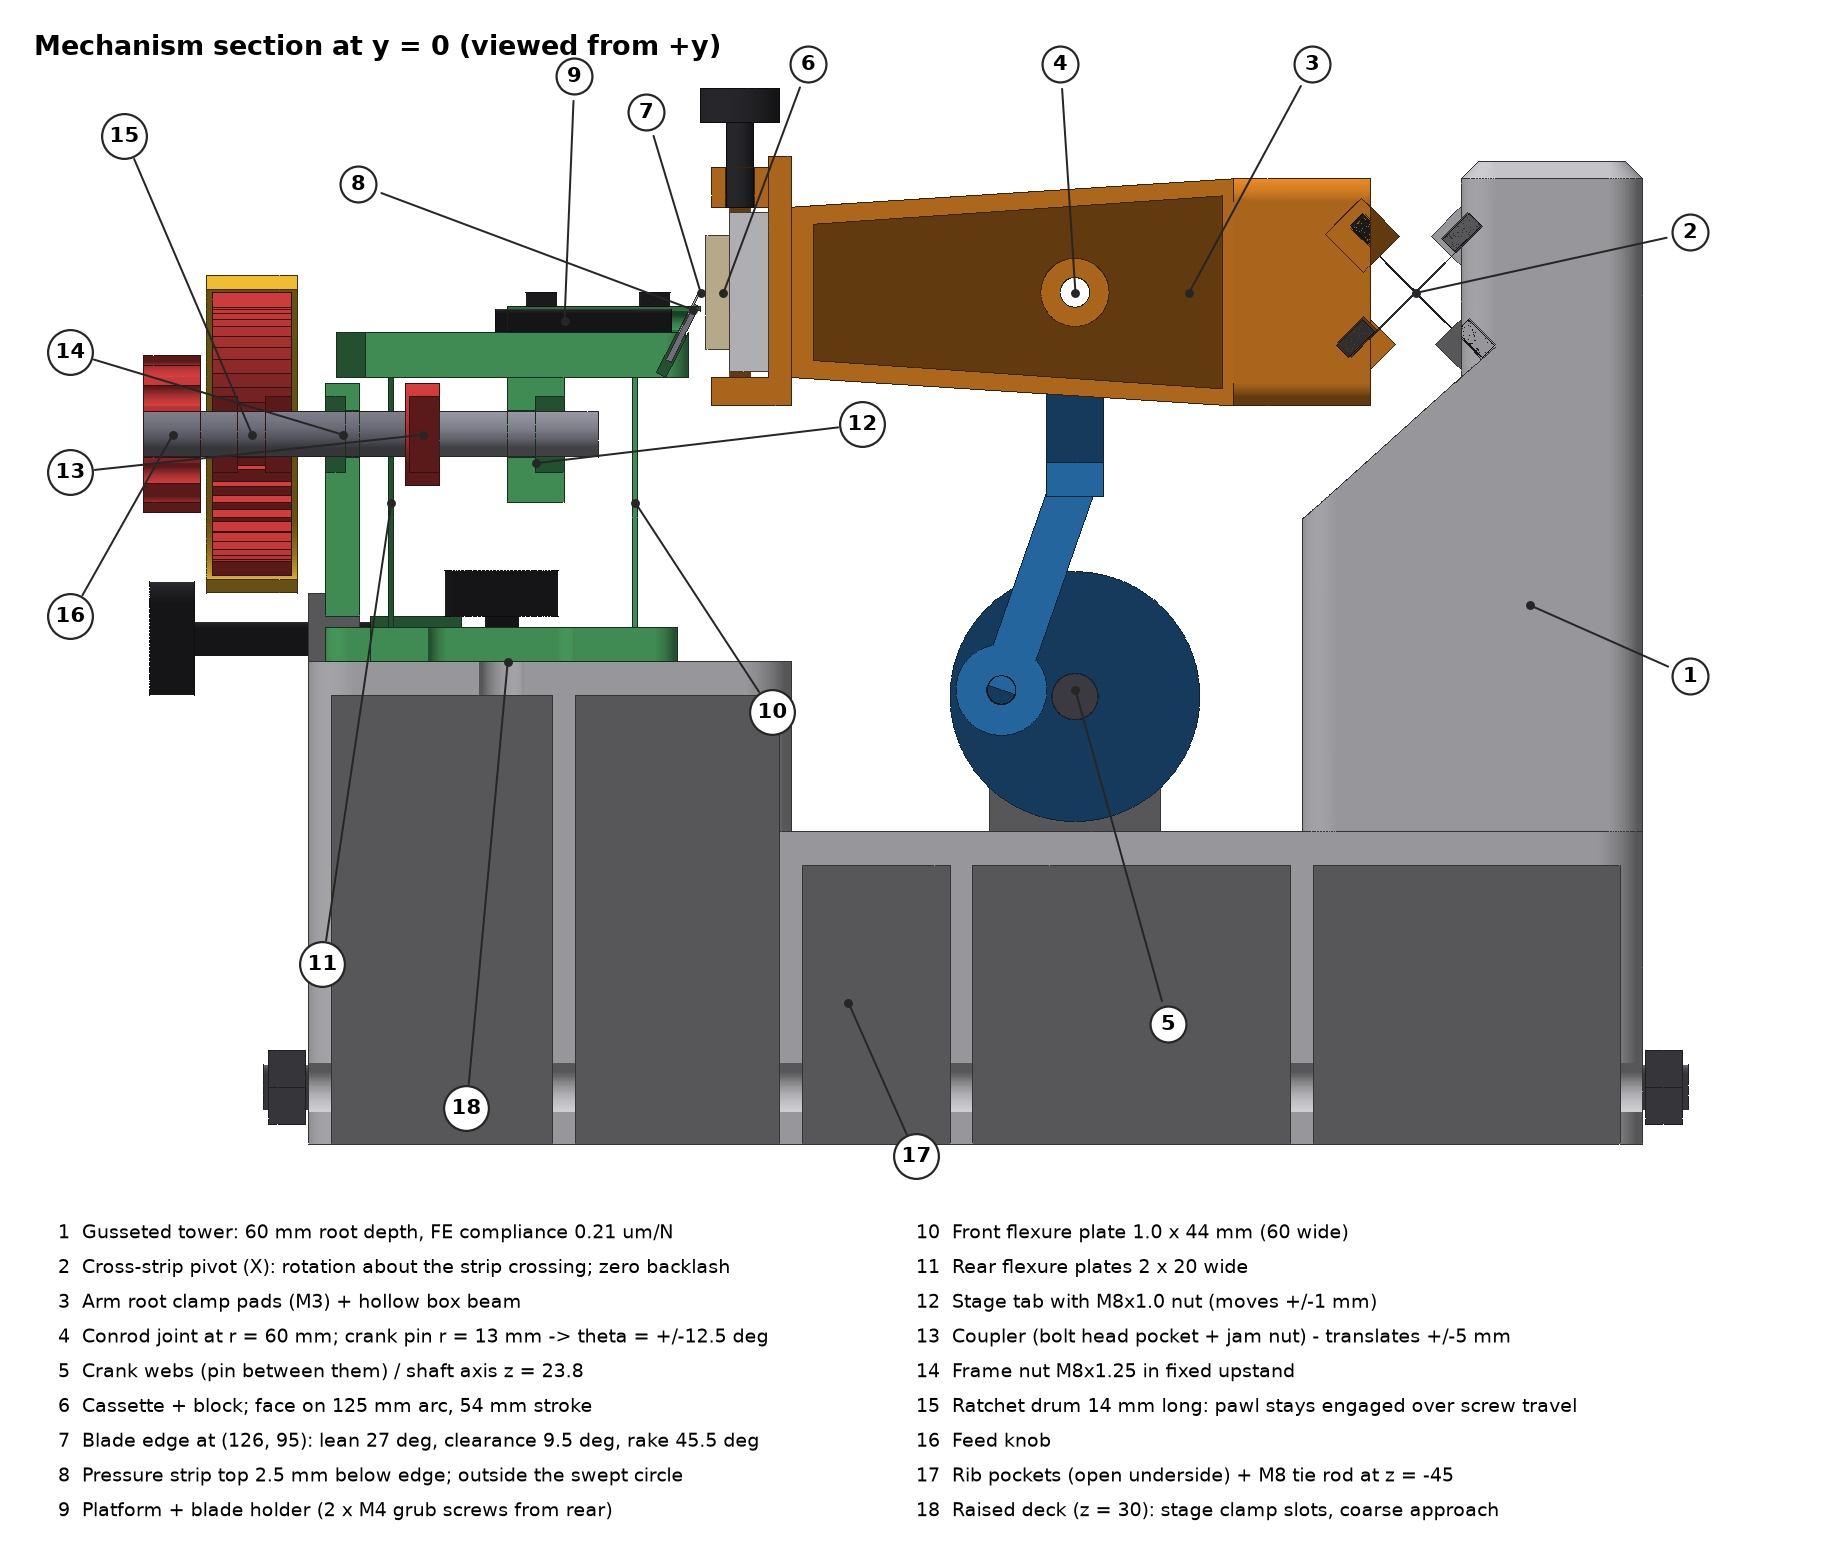
\includegraphics[width=\linewidth]{fig7_section_callouts.png}
\caption{Section through the mid-plane $y=0$, viewed from $+y$ (handwheel removed). The metrology loop runs from the blade edge (7) through the holder and platform (9), the flexure plates (10, 11), the stage nut tab (12), the differential screw and coupler (13), the frame nut (14), the deck and base (17, 18), the tower (1), the cross-strip pivot (2) and the arm (3) to the block face (6). The drive (crank webs (5), connecting rod (4)) hangs below the arm and is outside the loop.}
\label{fig:section}
\end{figure}

\FloatBarrier
\subsection{Drive train: handwheel to arm}
The handwheel (19; \SI{110}{\milli\metre}, five spokes, offset handle) turns a built-up crankshaft (18): two \SI{8}{\milli\metre} steel shaft stubs run in two 608 bearings in printed pillow blocks at $y=\pm50$\,mm, and are grub-screwed into two printed crank webs (\SI{44}{\milli\metre} diameter) that carry a \SI{5}{\milli\metre} crank pin at radius $r=\SI{13}{\milli\metre}$. The connecting rod (17) is a fork: its lower eye runs on the pin \emph{between} the two webs, and its two upper plates straddle the arm and pivot on a \SI{5}{\milli\metre} pin at $A$, \SI{60}{\milli\metre} from the arm pivot. Running the rod between the webs rather than beside a continuous shaft is what lets the pin pass below the shaft axis at the bottom of the stroke without the rod striking the shaft; this was a finding of the interference audit (Sec.~\ref{sec:audit}).

The crank centre $C=(60,\,23.8)$\,mm is placed exactly one connecting-rod length $\ell=\SI{71.2}{\milli\metre}$ below $A$'s mid-stroke position, so the two dead centres of the crank (pin directly above and below $C$) put $A$ at $z=95\pm13$\,mm and the swing is symmetric:
\begin{equation}
\sin\theta_{\max}=\frac{r}{r_{\mathrm{con}}}=\frac{13}{60}\quad\Rightarrow\quad\theta=\pm\ang{12.5},
\qquad
s=2L_{\mathrm{arm}}\sin\theta_{\max}=\SI{54.2}{\milli\metre}.
\end{equation}
For a general crank angle $\varphi$ the arm angle follows from loop closure $|A(\theta)-B(\varphi)|=\ell$ with $A=r_{\mathrm{con}}(\cos\theta,\sin\theta)+P$ and $B=C+r(\cos\varphi,\sin\varphi)$, solved numerically (Fig.~\ref{fig:mkin}b). The arm is horizontal when $\varphi_0=\arcsin\!\big(r/2\ell\big)=\ang{5.2}$, the rest pose used in the CAD. At 60~rpm the block face crosses the blade at 153--\SI{174}{\milli\metre\per\second} and the \SI{20}{\milli\metre} face is cut in \SI{118}{\milli\second} (Fig.~\ref{fig:mkin}c), i.e.\ the cutting-force pulse has its energy below $\sim$\SI{9}{\hertz}, far from the first structural mode (\SI{357}{\hertz}).

The torque the handwheel must supply is small: the pivot's elastic restoring torque peaks at \SI{0.058}{\newton\metre}, which through the \SI{60}{\milli\metre} arm joint, the rod and the \SI{13}{\milli\metre} crank becomes $\approx\SI{0.013}{\newton\metre}$ at the shaft, or \SI{0.23}{\newton} at the handle, imperceptible against the cutting force itself (0.6--\SI{2.4}{\newton} along the stroke).

\begin{figure}[!htbp]\centering
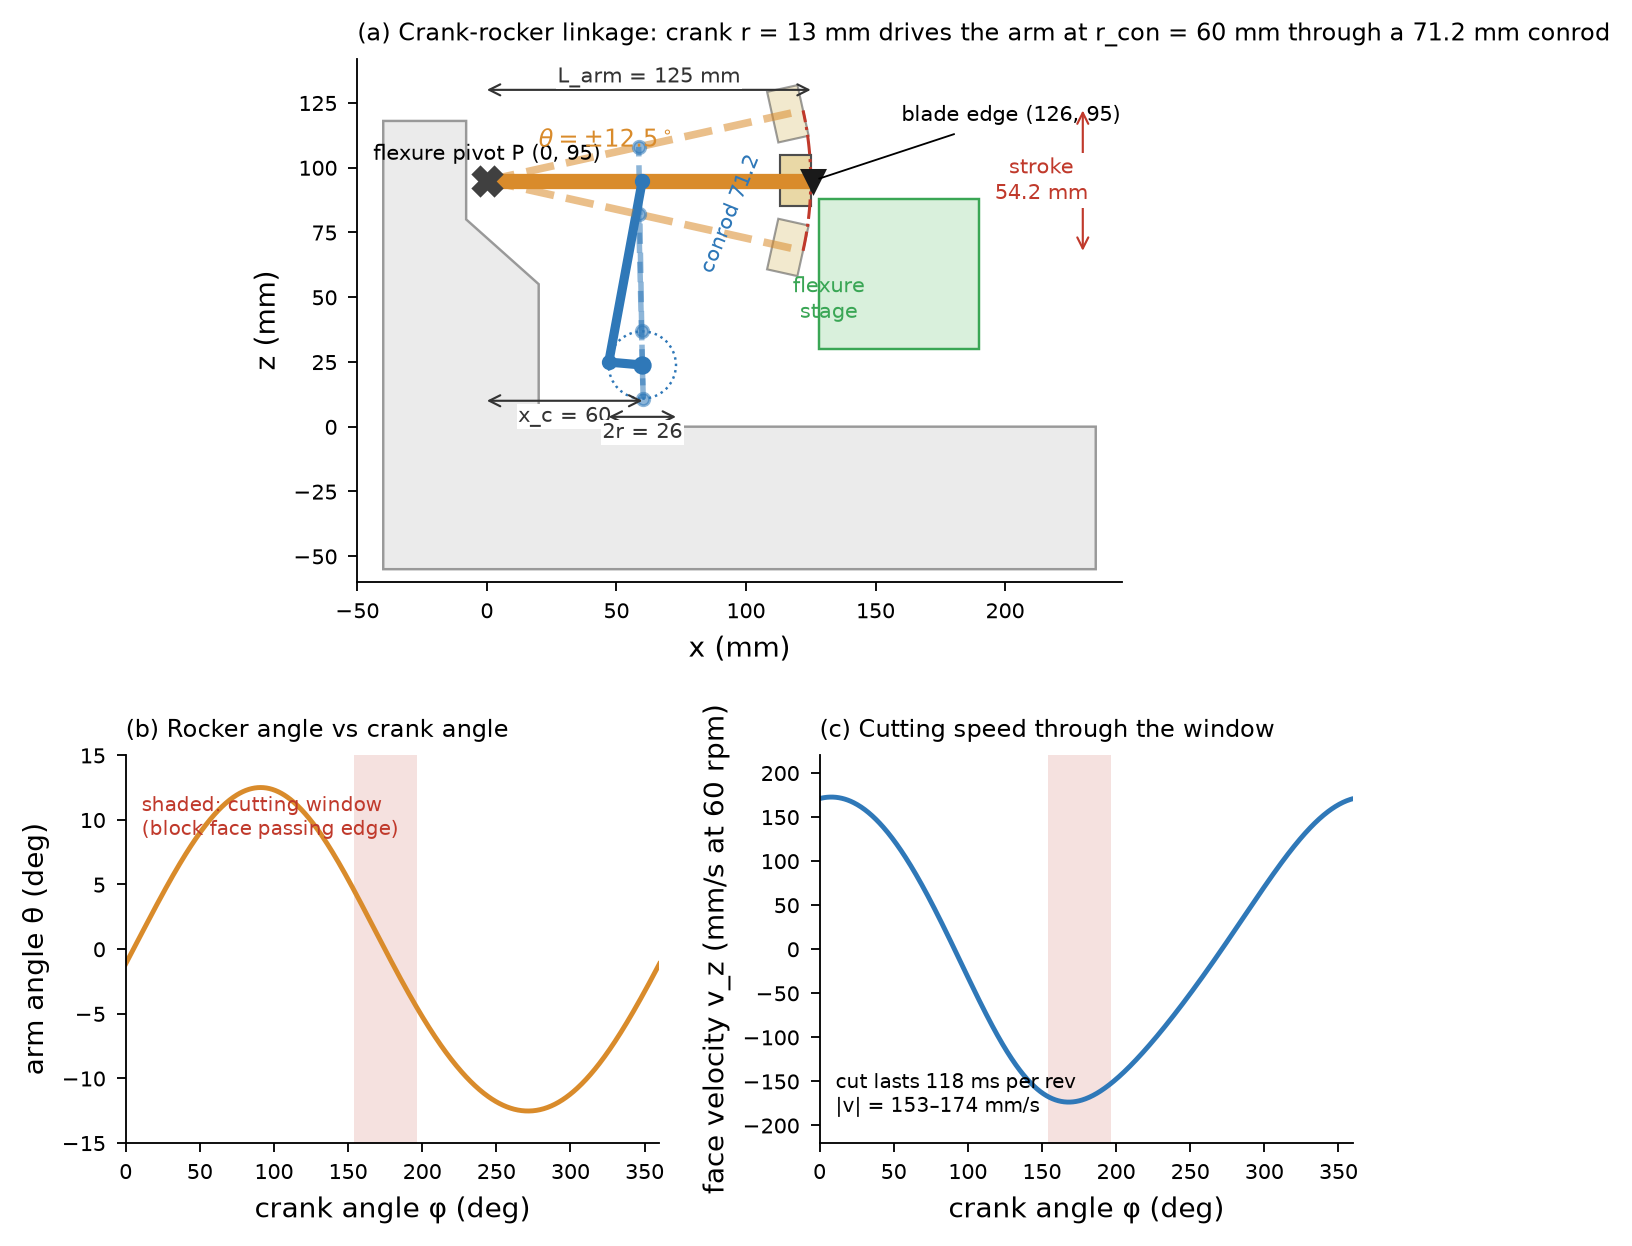
\includegraphics[width=\linewidth]{fig8_mech_kinematics.png}
\caption{Crank-rocker kinematics. (a)~Linkage to scale at mid-stroke (solid) and at the two extremes (dashed), with the block on the arm tip, the face arc (red dash-dot) and the stationary blade edge. (b)~Arm angle $\theta$ against crank angle $\varphi$; the shaded band is the cutting window, during which the \SI{20}{\milli\metre} face passes the edge ($|\theta|<\ang{4.6}$ on the down-stroke). (c)~Vertical face velocity at 60~rpm.}
\label{fig:mkin}
\end{figure}

\FloatBarrier
\subsection{The cut: blade and block geometry}
The blade (6) is a standard disposable low-profile blade ($80\times8\times\SI{0.25}{\milli\metre}$, \ang{35} included facet angle) clamped on the printed holder (7) behind a \SI{1.0}{\milli\metre} steel pressure strip, with the edge \SI{2.5}{\milli\metre} proud of the strip. The holder leans the blade back \ang{27} from the vertical block face. With a \ang{35} wedge the three angles at the edge (Fig.~\ref{fig:mblade}a) are therefore
\begin{equation}
\alpha_{\mathrm{clearance}} = 27^\circ-\tfrac{35^\circ}{2}=\ang{9.5},\qquad
\gamma_{\mathrm{rake}} = 90^\circ-27^\circ-\tfrac{35^\circ}{2}=\ang{45.5},\qquad
\alpha+\tfrac{\beta}{2}+\gamma=90^\circ .
\end{equation}
Because the block rides an arc of radius $L_{\mathrm{arm}}=\SI{125}{\milli\metre}$, the face tangent rotates with $\theta$ during the cut, and the instantaneous clearance sweeps $9.5\pm4.6^\circ$ (4.9--\ang{14.1}) across the face, inside the 3--\ang{15} window practitioners recommend~\citep{Bayley1955,Willis1995}. The same arc means the cut face is cylindrical, with sagitta
\begin{equation}
h=L_{\mathrm{arm}}-\sqrt{L_{\mathrm{arm}}^2-(b/2)^2}=\SI{401}{\micro\metre}\quad(b=\SI{20}{\milli\metre}),
\end{equation}
but since every stroke follows the same arc about the same (flexure-defined) centre, the arc is trimmed into the block once and successive sections (differences between successive arcs) are of uniform thickness (Fig.~\ref{fig:mblade}b). The pressure strip top sits \SI{2.5}{\milli\metre} below the edge along the blade, which places it just outside the block's swept circle; this is the geometric reason the \SI{2.0}{\milli\metre} overhang discussed in Sec.~\ref{sec:levers} is not available.

\begin{figure}[!htbp]\centering
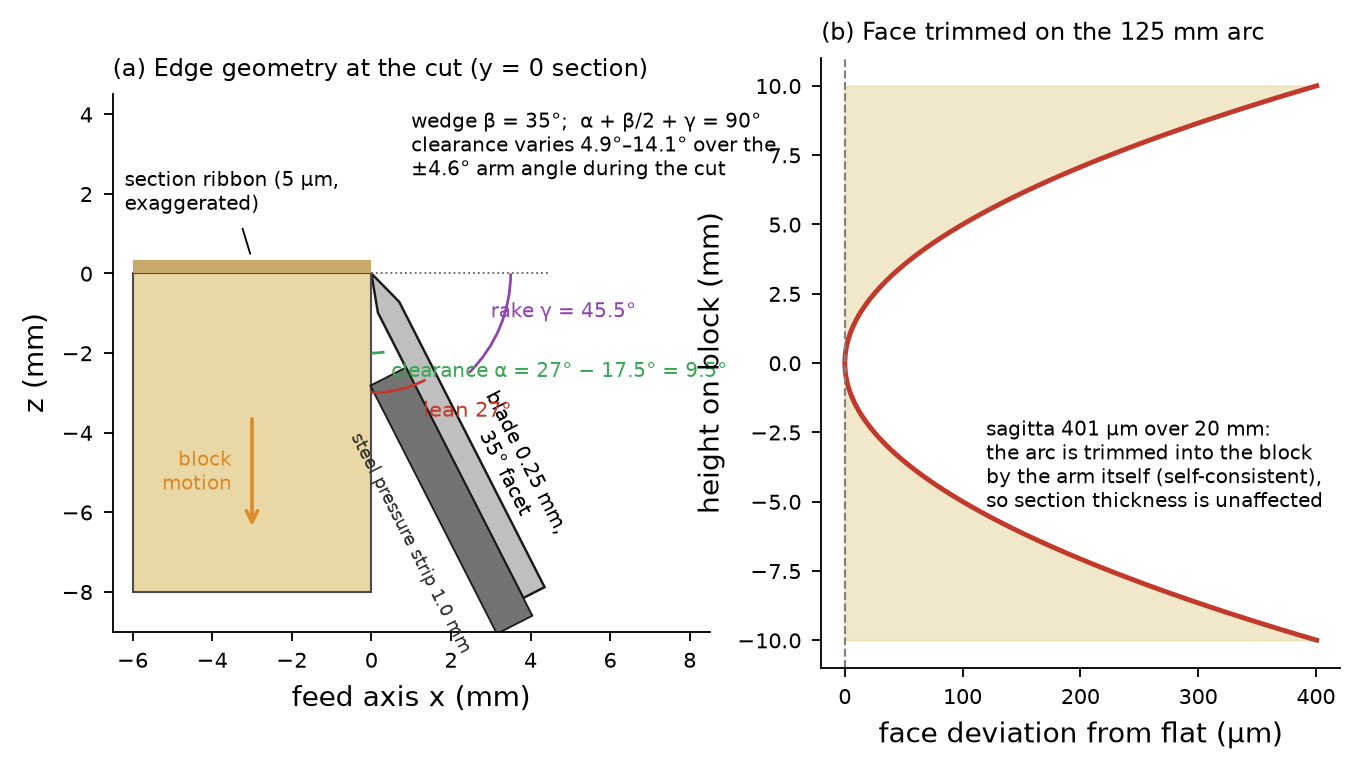
\includegraphics[width=\linewidth]{fig9_mech_blade.png}
\caption{Edge geometry. (a)~Mid-plane section at the cut: block (moving down), blade leaning \ang{27}, steel pressure strip, and the clearance, wedge and rake angles. (b)~Deviation of the arc-trimmed face from a plane over a \SI{20}{\milli\metre} block.}
\label{fig:mblade}
\end{figure}

\FloatBarrier
\subsection{The arm pivot: a cross-strip flexure}
The arm (3) is not on a pin or a bearing. Its root is held to the tower by three strips of \SI{0.20}{\milli\metre} feeler-gauge steel (2), two in one plane (10~mm wide each, at $y=\pm15$\,mm) and one in the perpendicular plane (20~mm wide, at $y=0$), crossing at the pivot axis with \SI{20}{\milli\metre} free length and clamped at both ends under printed pads with M3 screws (Fig.~\ref{fig:mpivot}a). The arm rotates by bending the strips; there is no sliding surface, so there is no backlash, no lubrication and no wear, and the restoring torque is elastic:
\begin{equation}
k_\theta=\sum_i\frac{E\,w_i t^3}{12\,L}=\SI{0.267}{\newton\metre\per\radian},\qquad
\sigma_{\max}=\frac{E\,t\,\theta_{\max}}{2L}=\SI{218}{\mega\pascal},\qquad
T_{\max}=k_\theta\theta_{\max}=\SI{0.058}{\newton\metre}.
\end{equation}
The stress is a factor 2 below the fatigue limit of hardened spring strip and 5 below yield. Along the feed axis the pivot is loaded in tension/compression of the strips and is very stiff (\SI{40}{\newton\per\micro\metre}; \SI{0.025}{\micro\metre\per\newton} in the loop). The price of a cross-strip pivot is a second-order shift of the rotation centre, $\approx0.1\,L\theta^2\approx\SI{95}{\micro\metre}$ at full swing~\citep{Wittrick1948,Haringx1949,SmithChetwynd2017}; because it is a deterministic function of $\theta$ it reshapes the arc slightly but is identical stroke to stroke, so it does not enter the thickness budget. Making the middle strip twice as wide as the outer two and placing it between them balances the two strip planes about $y=0$, so the pivot has no net twist about $z$ when the arm is loaded off-centre.

\FloatBarrier
\subsection{The feed train: differential screw, ratchet drum and selector}
The feed moves the blade, not the specimen. The blade stage (8) is a monolithic parallelogram: a platform on two \SI{1.0}{\milli\metre} PLA plates (front plate \SI{60}{\milli\metre} wide, rear pair $2\times20$\,mm) \SI{44}{\milli\metre} tall, so the platform translates along $x$ with no sliding joint. A tab hanging from the platform carries an M8$\times$1.0 nut; a fixed upstand on the stage foot carries an M8$\times$1.25 nut. One screw assembly (11) threads through both: an M8$\times$1.0 bolt in the tab, a printed coupler with a jam nut, and an M8$\times$1.25 rod in the frame nut, ending in the ratchet drum (12), two jam nuts and the feed knob (14). Turning the screw one revolution advances it \SI{1.25}{\milli\metre} through the frame nut, while the tab nut retreats \SI{1.00}{\milli\metre} along the screw (Fig.~\ref{fig:mscrew}a); the stage therefore moves by the difference,
\begin{equation}
\Delta x_{\mathrm{rev}}=p_1-p_2=1.25-1.00=\SI{0.25}{\milli\metre},\qquad
\Delta x_{\mathrm{tooth}}=\frac{\Delta x_{\mathrm{rev}}}{50}=\SI{5.0}{\micro\metre}.
\end{equation}
The flexure plates preload the tab against the screw (\SI{4.9}{\newton} at full travel), so the stage always rests on one thread flank and lead-screw backlash is removed. Three consequences follow from the differential principle. (i)~\emph{Reduction}: the screw body translates five times farther than the stage, so the \SI{14}{\milli\metre} drum, not a thin wheel, keeps the pawl engaged over the $\pm$\SI{5}{\milli\metre} screw excursion that accompanies the $\pm$\SI{1}{\milli\metre} stage travel (400 sections at \SI{5}{\micro\metre} per reset). (ii)~\emph{Tolerance}: only the \emph{difference} of the two pitches matters, so $\delta t/t=(\delta p_1-\delta p_2)/\SI{0.25}{\milli\metre}$; with 1\,\% independent local pitch errors this contributes \SI{0.37}{\micro\metre} (1~s.d.) at \SI{5}{\micro\metre} (Sec.~\ref{sec:levers}). (iii)~\emph{Resolution without precision parts}: both threads are ordinary rolled hardware; the micrometre-scale motion lives in steel while the printed parts only have to hold nuts.

The thickness selector (13) is a sector shield on the stage column that masks all but $k=1\ldots6$ teeth from the pawl finger, so each stroke advances $5k$\,\si{\micro\metre} (Fig.~\ref{fig:mscrew}b). The coarse approach after loading a new block is independent of the fine feed: the stage foot is clamped to the deck through $\pm$\SI{10}{\milli\metre} slots by two M6 knobs (9) and is pushed against an M6 screw in a side boss (10).

\begin{figure}[!htbp]\centering
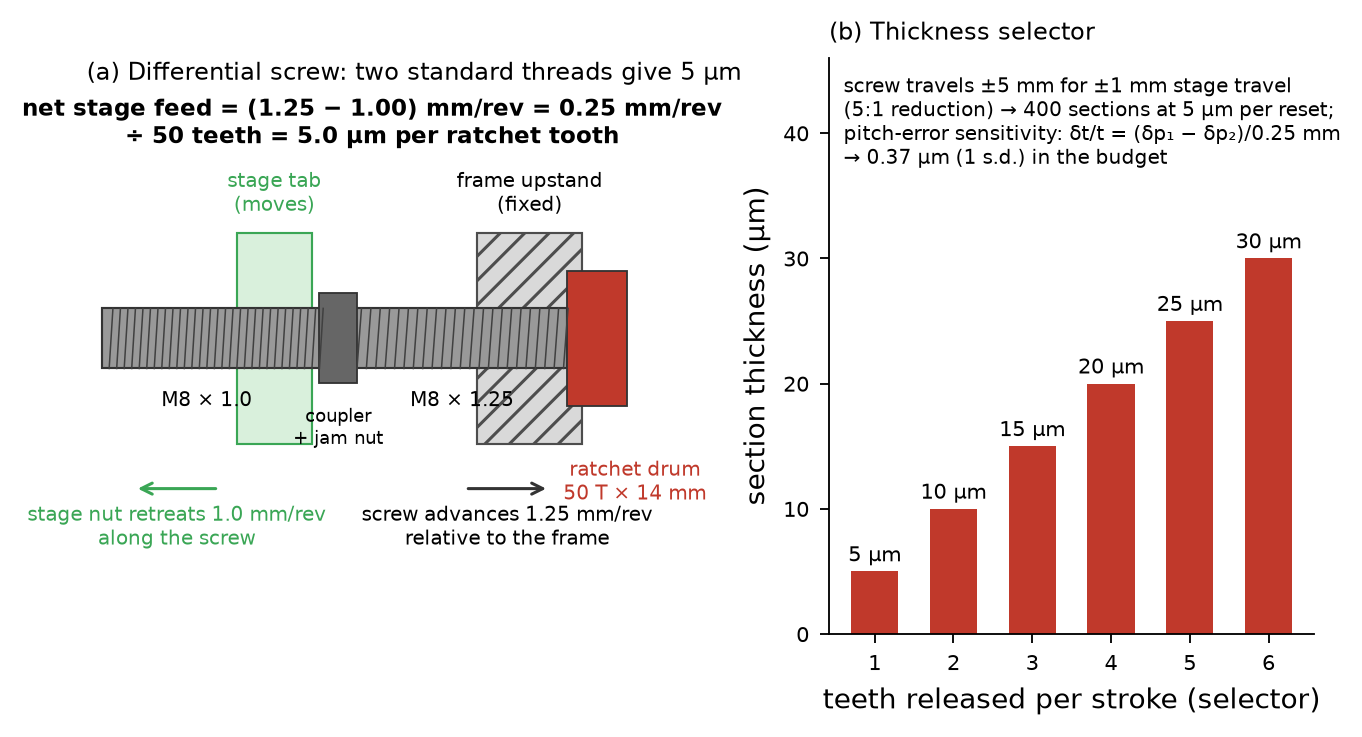
\includegraphics[width=\linewidth]{fig10_mech_screw.png}
\caption{Fine feed. (a)~Differential screw: the frame nut (M8$\times$1.25) and the stage-tab nut (M8$\times$1.0) move the stage by the pitch difference, \SI{0.25}{\milli\metre} per revolution, divided into 50 ratchet teeth. (b)~Selector settings and the resulting nominal section thickness.}
\label{fig:mscrew}
\end{figure}

\FloatBarrier
\subsection{Feed actuation: how one turn makes one section}
A vertical pawl rod (15) slides in a guide on the stage column; its finger rests on the drum teeth under gravity and a light spring. A striker bar (16) fixed to the arm reaches over the rod's flag. On the up-stroke, once the arm passes $\theta\approx\ang{6}$ (block \SI{13}{\milli\metre} clear of the edge) the bar lifts the rod, the finger slides back over the exposed teeth, and at the top of the stroke ($\theta=\ang{12.5}$, lift \SI{22}{\milli\metre}) it has ridden over $k$ teeth. As the arm comes back down past $\theta\approx\ang{6}$ the bar releases the rod; the finger drops behind the $k$th tooth and the rod's weight and spring turn the drum by $k\times\ang{7.2}$, advancing the blade $5k$\,\si{\micro\metre} toward the specimen \emph{before} the face reaches the edge (Fig.~\ref{fig:mtiming}). The feed is therefore complete and the drum is at rest during the cut; the ratchet never moves while the blade is in the block. Return-stroke retraction of the specimen (lifting it off the blade on the up-stroke) is not implemented; the arc geometry gives \SI{3.0}{\milli\metre} of natural retraction at the stroke ends but none at mid-face, so the back of the blade brushes the fresh face on the up-stroke as in the classical Cambridge rocker~\citep{Eaves1954}.

\begin{figure}[!htbp]\centering
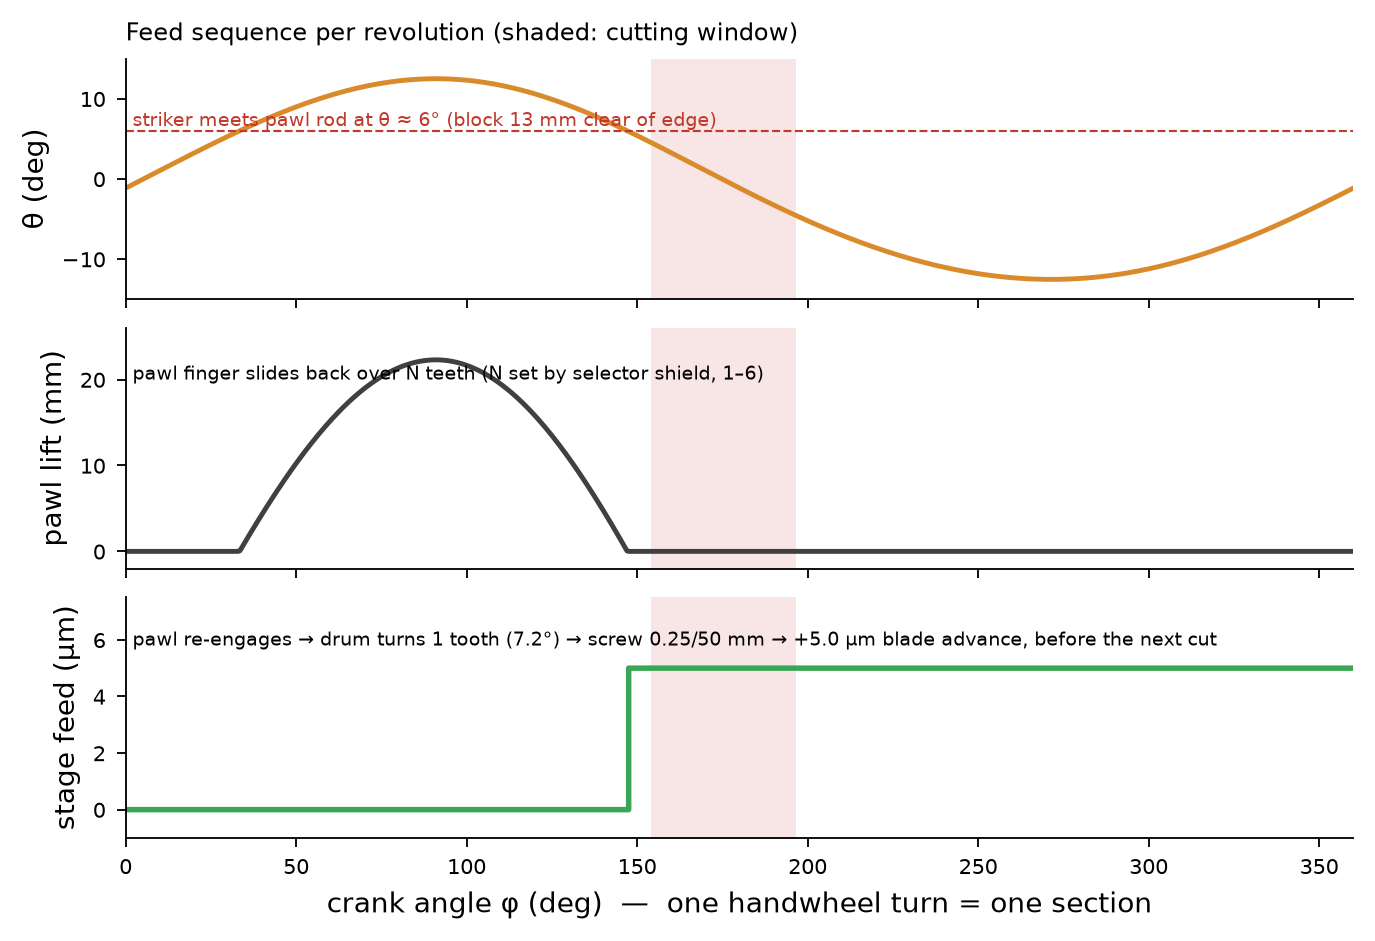
\includegraphics[width=\linewidth]{fig12_mech_timing.png}
\caption{Timing over one handwheel revolution: arm angle, pawl-rod lift and stage feed. The feed step occurs on the down-stroke before the cutting window (shaded).}
\label{fig:mtiming}
\end{figure}

\FloatBarrier
\subsection{The force path and why most of the machine does not matter}
Section thickness is set by the distance between the blade edge and the block face at the moment of the cut. Only parts on the closed path between those two points can change it; everything else (handwheel, crank, rod, drum, pawl) can be as flexible as PLA allows. Walking that loop in the section view (Fig.~\ref{fig:section}): edge~$\rightarrow$ blade overhang~$\rightarrow$ pressure strip and holder~$\rightarrow$ platform~$\rightarrow$ flexure plates (pitching about the nut)~$\rightarrow$ tab nut~$\rightarrow$ screw~$\rightarrow$ frame nut bedded in PLA~$\rightarrow$ upstand, deck, base~$\rightarrow$ tower~$\rightarrow$ strip pivot~$\rightarrow$ arm~$\rightarrow$ cassette clamp~$\rightarrow$ block. The feed-axis compliances add in series (Fig.~\ref{fig:mpivot}b):
\begin{equation}
C_{\mathrm{loop}}=\sum_i C_i=\SI{1.00}{\micro\metre\per\newton},\qquad k_{\mathrm{loop}}=1/C_{\mathrm{loop}}=\SI{1.0}{\newton\per\micro\metre}.
\end{equation}
A steady \SI{2}{\newton} feed-axis cutting force thus opens the loop by \SI{2}{\micro\metre}, but a steady deflection is cut into the block face and does not change the thickness; only its stroke-to-stroke \emph{variation} does (\SI{0.4}{\newton} s.d.~$\rightarrow$ \SI{0.40}{\micro\metre}). The three largest terms are the blade overhang (0.25), the frame between upstand and tower (0.21, FE) and the frame nut bedding in bare PLA (0.20), which is why a pressed brass insert for that nut is the cheapest upgrade (Sec.~\ref{sec:levers}).

\begin{figure}[!htbp]\centering
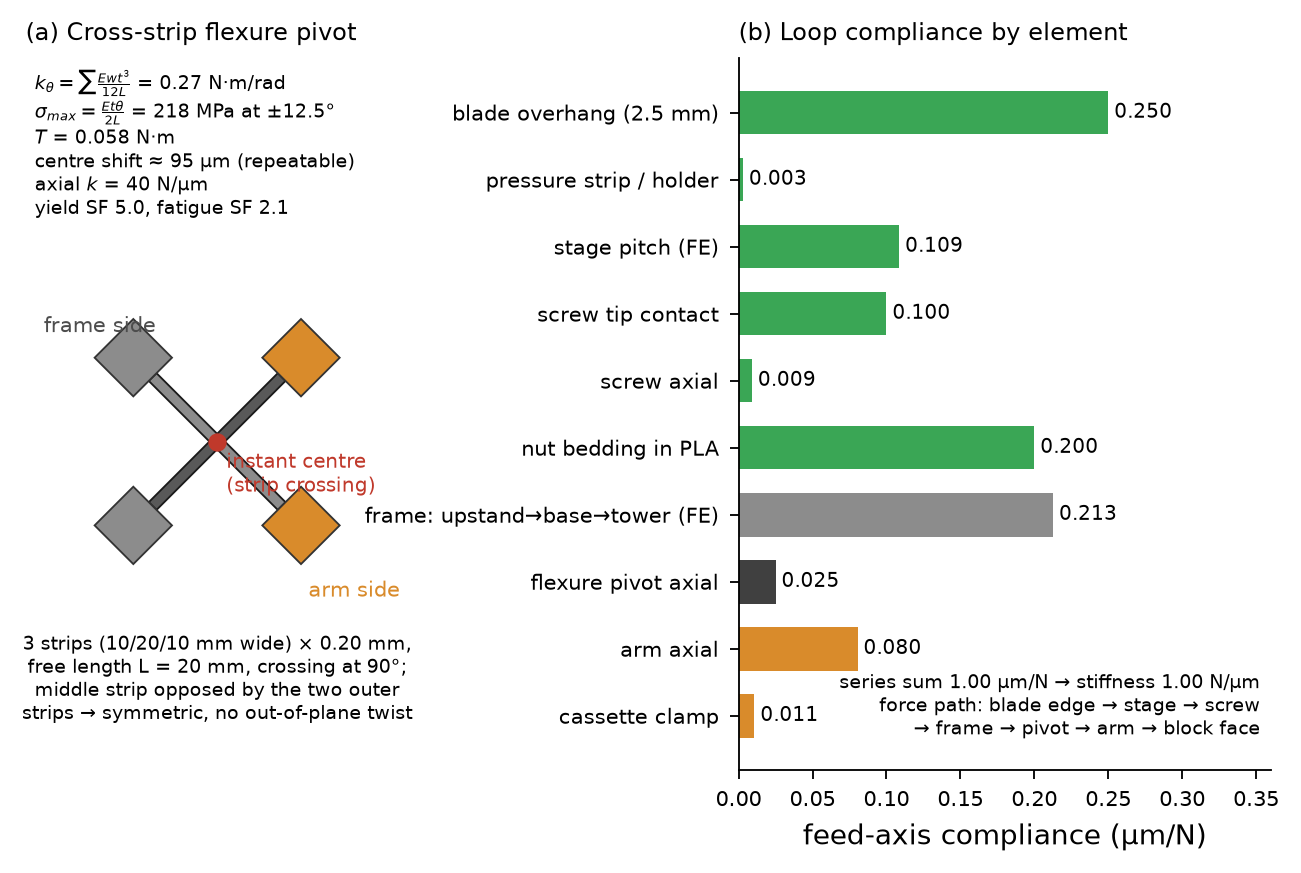
\includegraphics[width=\linewidth]{fig11_mech_pivot_loop.png}
\caption{(a)~Cross-strip pivot geometry and governing relations. (b)~Feed-axis compliance of each element of the metrology loop (green: blade stage group; grey: frame; dark: pivot; orange: arm and clamp).}
\label{fig:mpivot}
\end{figure}

\FloatBarrier
\subsection{Operating sequence}
\begin{enumerate}[nosep,leftmargin=*]
\item Clamp the cassette under the sliding jaw with the M5 thumbscrew (4); the block face must stand proud of the jaw.
\item Loosen the two M6 knobs (9), push the stage toward the block with the coarse screw (10) until the edge is $\sim$\SI{0.5}{\milli\metre} from the face, re-clamp.
\item Set the selector (13) to 6 teeth (\SI{30}{\micro\metre}) and turn the handwheel until the whole face is trimmed to the arc.
\item Set the selector to 1 tooth (\SI{5}{\micro\metre}); each further turn yields one \SI{5}{\micro\metre} section, which the previous section's wax edge carries off as a ribbon.
\item After $\sim$400 sections the stage reaches the end of its $\pm$\SI{1}{\milli\metre} travel: wind the feed knob (14) back 20 turns and repeat step~2.
\end{enumerate}

\FloatBarrier
\subsection{Design revisions driven by the interference audit}
\label{sec:audit}
A boolean interference audit of the assembly (12 crank angles over the full revolution, $\pm$\SI{5}{\milli\metre} screw travel, all part pairs) was re-run after every geometry change. It caught, and the design now reflects: the blade holder entering the specimen's swept circle (fixed by the \ang{27} lean and \SI{2.5}{\milli\metre} overhang); the striker bar passing through the pawl-rod body (bar moved outboard, flag added); the coarse-approach boss fouling the stage foot; the connecting-rod eye placed at the wrong crank position; the screw body translating five times the stage travel (drum ratchet, coupler gap, shield moved from the screw to the column); the connecting rod sweeping through a continuous crankshaft at the bottom of the stroke (built-up two-web crankshaft); and a \SI{1.2}{\milli\metre} offset of the crank centre that made the swing asymmetric ($-\ang{11.4}$ to $+\ang{13.7}$) rather than $\pm\ang{12.5}$ (crank centre lowered to $z=\SI{23.8}{\milli\metre}$). The only residual intersections are intended: pins in bores, strips in clamp pockets, the pawl tooth in the drum (\SI{16}{\milli\metre\cubed}), and the striker bar on the pawl flag between \ang{6} and \ang{12.5} of arm angle, which is the actuation itself.


\FloatBarrier
\section{Analysis methods}
\paragraph{Structural-loop model.} Each element between the blade edge and the specimen face was assigned a compliance along $x$ under a unit cutting force: axial compression of the arm and pivot strips, the FE-calibrated frame (tower + base) compliance, the FE-calibrated stage compliance, screw column, screw-tip and thread contacts, blade overhang bending, and clamp compressions. PLA $E=\SI{3.5}{\giga\pascal}$~\citep{Tymrak2014}, steel \SI{200}{\giga\pascal}.

\paragraph{Monte-Carlo thickness budget.} 20\,000 strokes were simulated with: independent 1\,\% pitch errors on both threads and a \SI{3}{\micro\metre} p-p periodic error; ratchet tooth-pitch error of \SI{0.05}{\milli\metre} (1~s.d.) on a \SI{60}{\milli\metre} diameter printed wheel; stroke-to-stroke cutting-force variation of \SI{0.4}{\newton} (1~s.d.) acting through the loop compliance; thermal drift over the \SI{1}{\second} stroke interval at \SI{1}{\kelvin} per \SI{30}{\minute} room drift; and \SI{0.1}{\micro\metre} pawl seating. The nominal cutting force (\SI{2}{\newton}) and its variation are assumptions (no absolute paraffin cutting-force measurement exists in the literature~\citep{Willis1995}), and Fig.~\ref{fig:stage}b shows the sensitivity.

\paragraph{Finite elements.} 2-D plane-stress linear elasticity (scikit-fem, quadratic triangles) of the stage cross-section and of the frame side-section, with out-of-plane widths represented by scaling $E$ per region. Verified against a cantilever benchmark (tip deflection \SI{97.3}{\milli\metre\per\newton} analytic vs 97.3 FE).

\paragraph{Modal estimates.} Lumped single-degree-of-freedom estimates for arm bending in the swing plane, stage $x$-motion and whole-loop $x$-motion.

\paragraph{Cost.} Printed-part cost from solid-modelled volume at US\$20/kg PLA (an upper bound; ribbed and infilled prints weigh less); hardware at typical online/hardware-store prices.

\FloatBarrier
\section{Results}
\subsection{Stiffness budget}
Total feed-axis compliance is \SI{1.00}{\micro\metre\per\newton} (stiffness \SI{1.00}{\newton\per\micro\metre}). The three largest terms are blade overhang (\SI{0.25}{\micro\metre\per\newton}), the frame (0.21, FE) and nut bedding in PLA (0.20); the pivot strips contribute only 0.02 (Fig.~\ref{fig:budget}a). With the original slender tower the total would have been \SI{1.62}{\micro\metre\per\newton}.

\begin{figure}[!htbp]\centering
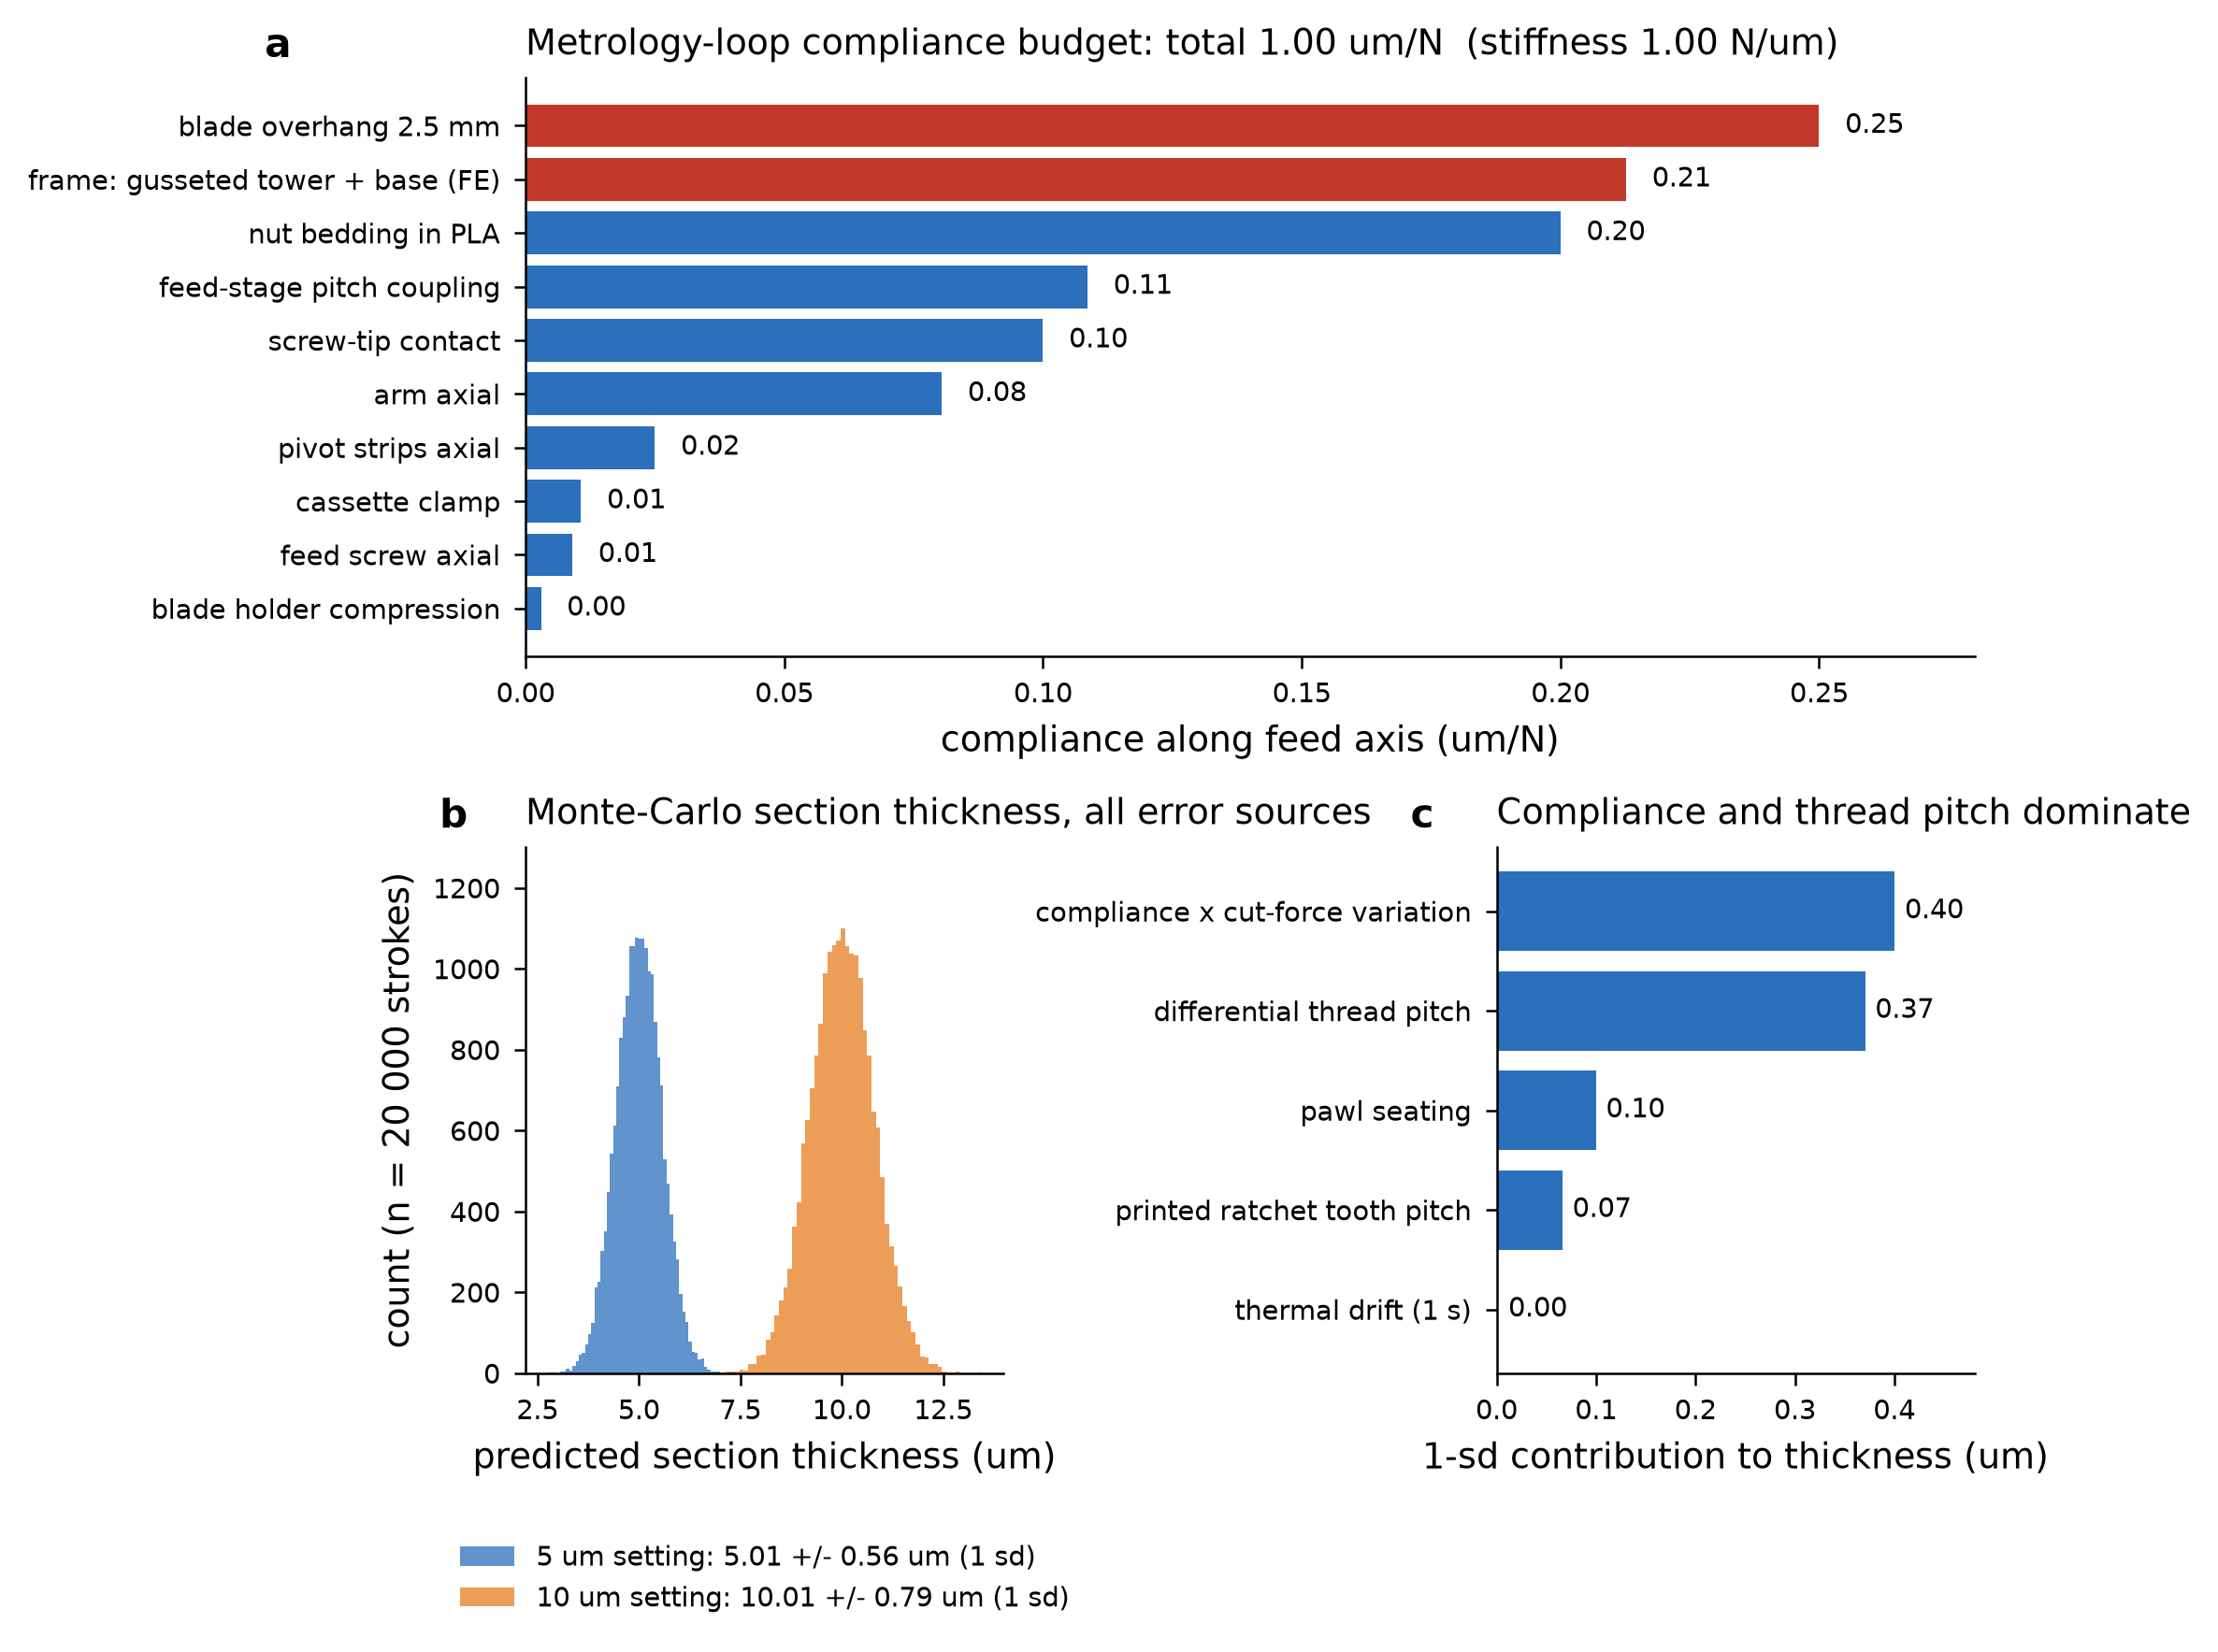
\includegraphics[width=\linewidth]{fig3_error_budget.png}
\caption{(a)~Compliance budget of the metrology loop. (b)~Monte-Carlo section thickness at the \SI{5}{\micro\metre} and \SI{10}{\micro\metre} settings ($n=20\,000$). (c)~1-s.d.\ contribution of each error source at the \SI{5}{\micro\metre} setting.}
\label{fig:budget}
\end{figure}

\subsection{Predicted section thickness}
At the \SI{5}{\micro\metre} setting the predicted section is $\mathbf{5.01\pm0.56}$\,\si{\micro\metre} (1~s.d.), 90\,\% interval 4.09--\SI{5.92}{\micro\metre}; at \SI{10}{\micro\metre}, $10.01\pm0.79$\,\si{\micro\metre}. Cutting-force variation through the loop compliance (\SI{0.40}{\micro\metre}) and differential-thread pitch scatter (\SI{0.37}{\micro\metre}) dominate; printed-ratchet error (\SI{0.07}{\micro\metre}) and thermal drift within a ribbon ($<$\SI{0.01}{\micro\metre}) are negligible (Fig.~\ref{fig:budget}c). With the slender tower the scatter would have been \SI{0.76}{\micro\metre} (Fig.~\ref{fig:stage}b). For context, direct measurement at 154 sites found more than two-thirds of sections from commercial rotary microtomes outside $\pm10\,\%$ of the dial setting~\citep{Fujisawa2026}; FlexTome's predicted 1-s.d.\ scatter is $\pm11\,\%$.

\subsection{Thermal behaviour}
The PLA loop expands \SI{10.6}{\micro\metre\per\kelvin}. This is irrelevant within a ribbon (strokes \SI{1}{\second} apart) but means the first sections after a temperature change or after mounting a new block will run thick or thin by several micrometres until trimmed, the same behaviour the Leica microtomy guide describes for a cold block, and handled by the same routine (trim, then section).

\subsection{Dynamics and chatter}
Estimated first modes: arm bending \SI{357}{\hertz}, whole-loop feed-axis \SI{504}{\hertz}, blade stage \SI{1.7}{\kilo\hertz}. A \SI{20}{\milli\metre} face is cut in \SI{118}{\milli\second}, so the cutting excitation is concentrated below $\sim$\SI{9}{\hertz}; no resonance-driven chatter is predicted. The rotational mode of the arm on its pivot ($\approx$\SI{4}{\hertz}) is the actuated degree of freedom and is constrained by the connecting rod.

\subsection{Cost and manufacturability}
\begin{table}[!htbp]\centering\small
\caption{Bill of materials (US\$).}
\begin{tabular}{@{}lr@{}}
\toprule
Category & Cost \\
\midrule
16 printed part types (20 pieces), \SI{1.36}{\litre} PLA (solid-modelled upper bound) & 33.69 \\
Hardware (feeler gauges, bearings, shaft, rods, nuts, screws, springs) & 24.10 \\
Consumables (one blade, adhesive, grease) & 2.60 \\
\midrule
\textbf{Total} & \textbf{60.39} \\
\bottomrule
\end{tabular}
\end{table}
Against US\$8\,995--22\,690 new and US\$2\,100--7\,950 used, this is a $>99\,\%$ and $>97\,\%$ reduction respectively. The largest part (frame, $235\times150\times173$\,mm) fits an Ender-3-class \SI{235}{\milli\metre} bed (or is split at the deck step for smaller printers); all other parts fit a \SI{180}{\milli\metre} bed. No machining is required; the only cutting operations are shearing feeler-gauge strips to length and cutting threaded rod.

\subsection{Cutting-force bound, improvement levers and the entry transient}
\label{sec:levers}
Because no absolute paraffin cutting force has been published, the $2\pm0.4$\,\si{\newton} assumption was bracketed with the pressing-and-slicing fracture model~\citep{Atkins2004}: with a fracture work $R=20$--\SI{80}{\joule\per\metre\squared}, wax yield stress 1--\SI{3}{\mega\pascal}, a \ang{35} facet and friction coefficient 0.3, a $\SI{5}{\micro\metre}\times\SI{25}{\milli\metre}$ cut requires 0.6--\SI{2.4}{\newton} along the stroke and only 0.23--\SI{0.86}{\newton} along the feed axis ($\leq$\SI{1.3}{\newton} for a dulled blade with doubled friction). The feed-axis force that drives thickness error is therefore likely below the \SI{2}{\newton} assumed, and the \SI{0.4}{\newton} (1~s.d.) variation is conservative; at \SI{0.2}{\newton} the predicted scatter falls to \SI{0.44}{\micro\metre}.

Of the two levers identified by the budget, reducing blade overhang from 2.5 to \SI{2.0}{\milli\metre} is \emph{not} available at the chosen geometry: the \SI{1.0}{\milli\metre} pressure strip's top edge would then sit \SI{0.09}{\milli\metre} inside the specimen's swept circle (it needs a \SI{0.8}{\milli\metre} strip or a \ang{29} lean). Seating the frame nut in a pressed brass insert instead of bare PLA is available and reduces loop compliance from 1.00 to \SI{0.85}{\micro\metre\per\newton} (scatter $0.56\rightarrow$\SI{0.52}{\micro\metre}).

Within a single section, the cutting force rises over the $\sim$\SI{0.5}{\milli\metre} entry chamfer of the block face in $\sim$\SI{3}{\milli\second}. Driving the \SI{504}{\hertz}, 3\,\%-damped loop with that ramp gives an 18\,\% dynamic overshoot (\SI{0.36}{\micro\metre} on a \SI{2}{\micro\metre} quasi-static deflection) that rings down within \SI{42}{\milli\second} of the \SI{118}{\milli\second} cut, bounding within-section thickness non-uniformity from this source to $\approx$\SI{0.4}{\micro\metre} over the first \SI{7}{\milli\metre} of the face.

\FloatBarrier
\section{Discussion}
\paragraph{What the analysis establishes.} The predicted $5.0\pm0.6$\,\si{\micro\metre} is a model result, not a measurement. Its value is that it identifies, quantitatively, what limits a printed microtome: not feed resolution (the steel differential screw delivers \SI{5}{\micro\metre} trivially) but loop stiffness against cutting-force variation, and within that, blade overhang, tower bending and nut bedding. The frame FE is the clearest lesson of the study: a beam-theory budget built on an idealised tower section under-predicted tower compliance eight-fold and credited the tie rods with a stiffening they do not provide; the FE both exposed the error and pointed to the fix (a gusset within the footprint). The next lever is seating the frame nut in a brass insert (Section~\ref{sec:levers}); reducing blade overhang below \SI{2.5}{\milli\metre} requires a thinner pressure strip or a steeper lean.

\paragraph{Relation to prior art.} The Darwin rocker already combined arm, screw and ratchet; what it lacked was a bearing that a printed machine could reproduce. Replacing its hardened steel knife-edge or journal pivot with crossed feeler-gauge strips removes the one component that required a machine shop. The differential screw is a textbook element~\citep{SmithChetwynd2017} but has not previously been reported in a microtome, where it allows the \SI{5}{\micro\metre} increment to come from two hardware-store threads rather than a micrometer spindle. The parallelogram blade stage follows the OpenFlexure precedent that FDM compliant mechanisms achieve micron-scale repeatability~\citep{Sharkey2016}.

\paragraph{Limitations and risks.}
\begin{enumerate}[nosep]
\item \emph{Cutting force is assumed.} The $2\pm0.4$\,\si{\newton} figure is an engineering estimate bracketed by fracture mechanics; no measured value exists. Doubling the variation to \SI{0.8}{\newton} raises scatter to \SI{1.04}{\micro\metre}. A load-cell measurement on the build is therefore both a validation step and a contribution in its own right.
\item \emph{No specimen retraction on the return stroke.} The face passes the edge on the upstroke flush with it. Basic manual rotary microtomes without retraction are used routinely, but knife lines are possible; a 50--\SI{100}{\micro\metre} retraction cam acting on the stage is a planned addition.
\item \emph{Cylindrical block face.} The \SI{0.40}{\milli\metre} sagitta over \SI{20}{\milli\metre} is the rocker's known property; sections flatten on the water bath. Block height is limited to $\sim$\SI{25}{\milli\metre} by the clearance-angle variation.
\item \emph{PLA creep and humidity.} The stage flexure is loaded only while displaced from neutral ($\leq$\SI{5}{\newton}, \SI{5.4}{\mega\pascal}); the user returns the screw to centre after each block. PETG/ASA or 100\,\% infill at \SI{0.1}{\milli\metre} layers reduce creep further~\citep{Waseem2020}.
\item \emph{Thread backlash.} The flexure preload and the unidirectional cutting load keep the nut flanks engaged; reversing the feed requires re-trimming, as on any manual microtome.
\item \emph{Blade clamping.} Two M4 grub screws from behind against a \SI{1}{\milli\metre} steel pressure strip is simpler than a commercial clamp; blade seating repeatability must be verified.
\end{enumerate}

\paragraph{Broader impact.} A \$60 microtome does not create a pathology service; it needs embedding, staining, a microscope and, above all, a pathologist or a telepathology link. But it removes the single highest-cost mechanical item from the chain, and does so with a device that a hospital workshop or a school with a desktop printer can build and repair. Combined with the OpenFlexure microscope, it brings the entire physical chain from block to image under US\$300.

\FloatBarrier
\section{Validation plan (for the physical build)}
\begin{enumerate}[nosep]
\item \textbf{Print and assemble} (frame 100\,\% infill in the pivot and deck regions, \SI{0.2}{\milli\metre} layers; stage flexure 100\,\% infill, \SI{0.1}{\milli\metre} layers, plates printed vertically). Record print mass and time.
\item \textbf{Static loop stiffness.} Apply 0.5--\SI{3}{\newton} to the block face along $x$ with a hanging mass over a pulley; read displacement with a \SI{1}{\micro\metre} dial indicator at the blade edge. Target $\geq$\SI{0.8}{\newton\per\micro\metre}. Compare to the budget element by element by moving the indicator.
\item \textbf{Feed calibration.} Advance 50 teeth (one revolution) and measure $250\pm5$\,\si{\micro\metre} stage travel; repeat 10$\times$ for pitch-error scatter.
\item \textbf{Section thickness.} (a)~Block-consumption method: dial indicator on the trimmed face before and after 100 sections at \SI{5}{\micro\metre}. (b)~Gravimetric: weigh ribbons of 20 sections of known face area (paraffin density \SI{0.90}{\gram\per\centi\metre\cubed}). (c)~Optical: measure 20 individual sections with a confocal/interference microscope if available, following~\citet{Fujisawa2026}. Report mean, s.d.\ and the fraction within $\pm10\,\%$.
\item \textbf{Cutting force.} Mount a \SI{5}{\newton} load cell under the stage foot; record force vs crank angle over 50 strokes to replace the assumed $2\pm0.4$\,\si{\newton}.
\item \textbf{Section quality.} Cut \SI{5}{\micro\metre} ribbons from standard test blocks (liver, kidney, skin) on FlexTome and a commercial microtome; H\&E stain; blinded scoring (compression, chatter, knife lines, folds) by two histotechnologists.
\item \textbf{Durability.} 10\,000 strokes ($\approx$\SI{3}{\hour} at 60~rpm, motor-driven), then repeat steps 2--4.
\end{enumerate}

\FloatBarrier
\section{Conclusion}
A rocking microtome whose precision-critical joints are flexures and whose micrometre feed chain is entirely steel can be built from printed PLA and hardware-store parts for US\$60. The FE-checked design analysis predicts $5.0\pm0.6$\,\si{\micro\metre} sections at a loop stiffness of \SI{1.0}{\newton\per\micro\metre}, with stiffness, not feed resolution, as the limiting quantity, and identifies blade overhang, tower bending and nut seating as the levers for improvement. The complete CAD, analysis code and validation protocol are released with this report so that the prediction can be tested, and the design iterated, by anyone with a desktop printer.

\section*{Data and code availability}
\texttt{flextome\_assembly.step} (full assembly), \texttt{flextome\_stl\_parts.zip} (30 component STLs + \texttt{parts.json}), \texttt{flextome\_cad.py} (parametric CadQuery source), \texttt{flextome\_design.py} (analytic model and Monte-Carlo), \texttt{fea\_stage.py}, \texttt{fea\_frame.py} (finite-element models), \texttt{make\_figures.py}, \texttt{flextome\_bom.csv}, \texttt{references.csv} and \texttt{evidence\_summary.md} (verified literature base).

\bibliographystyle{unsrtnat}
\bibliography{flextome}
\end{document}
